% !TeX spellcheck = pl_PL
%%%%%%%%%%%%%%%%%%%%%%%%%%%%%%%%%%%%%%%%%%%
%                                        %
% Szablon pracy dyplomowej inzynierskiej %
% zgodny  z aktualnymi  przepisami  SZJK %
%                                        %
%%%%%%%%%%%%%%%%%%%%%%%%%%%%%%%%%%%%%%%%%%
%                                        %
%  (c) Krzysztof Simiński, 2018-2023     %
%                                        %
%%%%%%%%%%%%%%%%%%%%%%%%%%%%%%%%%%%%%%%%%%
%                                        %
% Najnowsza wersja szablonów jest        %
% podstępna pod adresem                  %
% github.com/ksiminski/polsl-aei-theses  %
%                                        %
%%%%%%%%%%%%%%%%%%%%%%%%%%%%%%%%%%%%%%%%%%
%
%
% Projekt LaTeXowy zapewnia odpowiednie formatowanie pracy,
% zgodnie z wymaganiami Systemu zapewniania jakości kształcenia.
% Proszę nie zmieniać ustawień formatowania (np. fontu,
% marginesów, wytłuszczeń, kursywy itd. ).
%
% Projekt można kompilować na kilka sposobów.
%
% 1. kompilacja pdfLaTeX
%
% pdflatex main
% bibtex   main
% pdflatex main
% pdflatex main
%
%
% 2. kompilacja XeLaTeX
%
% Kompilatacja przy użyciu XeLaTeXa różni się tym, że na stronie
% tytułowej używany jest font Calibri. Wymaga to jego uprzedniego
% zainstalowania.
%
% xelatex main
% bibtex  main
% xelatex main
% xelatex main
%
%
%%%%%%%%%%%%%%%%%%%%%%%%%%%%%%%%%%%%%%%%%%%%%%%%%%%%%
% W przypadku pytań, uwag, proszę pisać na adres:   %
%      krzysztof.siminski(małpa)polsl.pl            %
%%%%%%%%%%%%%%%%%%%%%%%%%%%%%%%%%%%%%%%%%%%%%%%%%%%%%
%
% Chcemy ulepszać szablony LaTeXowe prac dyplomowych.
% Wypełniając ankietę spod poniższego adresu pomogą
% Państwo nam to zrobić. Ankieta jest całkowicie
% anonimowa. Dziękujemy!


% https://docs.google.com/forms/d/e/1FAIpQLScyllVxNKzKFHfILDfdbwC-jvT8YL0RSTFs-s27UGw9CKn-fQ/viewform?usp=sf_link
%
%%%%%%%%%%%%%%%%%%%%%%%%%%%%%%%%%%%%%%%%%%%%%%%%%%%%%%%%%%%%%%%%%%%%%%%%%

%%%%%%%%%%%%%%%%%%%%%%%%%%%%%%%%%%%%%%%%%%%%%%%
%                                             %
% PERSONALIZACJA PRACY – DANE PRACY           %
%                                             %
%%%%%%%%%%%%%%%%%%%%%%%%%%%%%%%%%%%%%%%%%%%%%%%

% Proszę wpisać swoje dane w poniższych definicjach.

% TODO
% dane autora
\newcommand{\FirstNameAuthor}{Jakub}
\newcommand{\SurnameAuthor}{Sibik}
\newcommand{\IdAuthor}{300420}   % numer albumu  (bez $\langle$ i $\rangle$)

% drugi autor:
%\newcommand{\FirstNameCoauthor}{Imię}   % Jeżeli jest drugi autor, to tutaj należy podać imię.
%\newcommand{\SurnameCoauthor}{Nazwisko} % Jeżeli jest drugi autor, to tutaj należy podać nazwisko.
%\newcommand{\IdCoauthor}{$\langle$wpisać właściwy$\rangle$}  % numer albumu drugiego autora (bez $\langle$ i $\rangle$)
% Gdy nie ma drugiego autora, należy zostawić poniższe definicje puste, jak poniżej. Gdy jest drugi autor, należy zakomentować te linie.
\newcommand{\FirstNameCoauthor}{} % Jeżeli praca ma tylko jednego autora, to dane drugiego autora zostają puste.
\newcommand{\SurnameCoauthor}{}   % Jeżeli praca ma tylko jednego autora, to dane drugiego autora zostają puste.
\newcommand{\IdCoauthor}{}  % Jeżeli praca ma tylko jednego autora, to dane drugiego autora zostają puste.
%%%%%%%%%%

\newcommand{\Supervisor}{dr inż. Łukasz Wyciślik}     % dane promotora (bez $\langle$ i $\rangle$)
\newcommand{\Title}{System do monitorowania położenia geoprzestrzennego obiektów}           % tytuł pracy po polsku
\newcommand{\TitleAlt}{Thesis title in English}                     % thesis title in English
\newcommand{\Program}{Informatyka}            % kierunek studiów  (bez $\langle$ i $\rangle$)
\newcommand{\Specialisation}{Informatyczne Systemy Mobilne i Przemysłowe}     % specjalność  (bez $\langle$ i $\rangle$)
\newcommand{\Departament}{Informatyki Stosowanej}        % katedra promotora  (bez $\langle$ i $\rangle$)

% Jeżeli został wyznaczony promotor pomocniczy lub opiekun, proszę go/ją wpisać ...
%\newcommand{\Consultant}{$\langle$stopień naukowy imię i nazwisko$\rangle$} % dane promotora pomocniczego, opiekuna (bez $\langle$ i $\rangle$)
% ... w przeciwnym razie proszę zostawić puste miejsce jak poniżej:
\newcommand{\Consultant}{} % brak promotowa pomocniczego / opiekuna

% koniec fragmentu do modyfikacji
%%%%%%%%%%%%%%%%%%%%%%%%%%%%%%%%%%%%%%%%%%


%%%%%%%%%%%%%%%%%%%%%%%%%%%%%%%%%%%%%%%%%%%%%%%
%                                             %
% KONIEC PERSONALIZACJI PRACY                 %
%                                             %
%%%%%%%%%%%%%%%%%%%%%%%%%%%%%%%%%%%%%%%%%%%%%%%

%%%%%%%%%%%%%%%%%%%%%%%%%%%%%%%%%%%%%%%%


%%%%%%%%%%%%%%%%%%%%%%%%%%%%%%%%%%%%%%%%%%%%%%%
%                                             %
% PROSZĘ NIE MODYFIKOWAĆ PONIŻSZYCH USTAWIEŃ! %
%                                             %
%%%%%%%%%%%%%%%%%%%%%%%%%%%%%%%%%%%%%%%%%%%%%%%



\documentclass[a4paper,twoside,12pt]{book}
\usepackage[utf8]{inputenc}                                      
\usepackage[T1]{fontenc}  
\usepackage{amsmath,amsfonts,amssymb,amsthm}
\usepackage[british,polish]{babel} 
\usepackage{indentfirst}
\usepackage{xurl}
\usepackage{xstring}
\usepackage{ifthen}



\usepackage{ifxetex}

\ifxetex
	\usepackage{fontspec}
	\defaultfontfeatures{Mapping=tex—text} % to support TeX conventions like ``——-''
	\usepackage{xunicode} % Unicode support for LaTeX character names (accents, European chars, etc)
	\usepackage{xltxtra} % Extra customizations for XeLaTeX
\else
	\usepackage{lmodern}
\fi



\usepackage[margin=2.5cm]{geometry}
\usepackage{graphicx} 
\usepackage{hyperref}
\usepackage{booktabs}
\usepackage{tikz}
\usepackage{pgfplots}
\usepackage{mathtools}
\usepackage{geometry}
\usepackage{subcaption}   % subfigures
\usepackage[page]{appendix} % toc,
\renewcommand{\appendixtocname}{Dodatki}
\renewcommand{\appendixpagename}{Dodatki}
\renewcommand{\appendixname}{Dodatek}

\usepackage{csquotes}
\usepackage[natbib=true,backend=bibtex,maxbibnames=99]{biblatex}  % kompilacja bibliografii BibTeXem
%\usepackage[natbib=true,backend=biber,maxbibnames=99]{biblatex}  % kompilacja bibliografii Biberem
\bibliography{biblio/biblio}

\usepackage{ifmtarg}   % empty commands  

\usepackage{setspace}
\onehalfspacing


\frenchspacing



%%%% TODO LIST GENERATOR %%%%%%%%%

\usepackage{color}
\definecolor{brickred}      {cmyk}{0   , 0.89, 0.94, 0.28}

\makeatletter \newcommand \kslistofremarks{\section*{Uwagi} \@starttoc{rks}}
  \newcommand\l@uwagas[2]
    {\par\noindent \textbf{#2:} %\parbox{10cm}
{#1}\par} \makeatother


\newcommand{\ksremark}[1]{%
{%\marginpar{\textdbend}
{\color{brickred}{[#1]}}}%
\addcontentsline{rks}{uwagas}{\protect{#1}}%
}

\newcommand{\comma}{\ksremark{przecinek}}
\newcommand{\nocomma}{\ksremark{bez przecinka}}
\newcommand{\styl}{\ksremark{styl}}
\newcommand{\ortografia}{\ksremark{ortografia}}
\newcommand{\fleksja}{\ksremark{fleksja}}
\newcommand{\pauza}{\ksremark{pauza `--', nie dywiz `-'}}
\newcommand{\kolokwializm}{\ksremark{kolokwializm}}
\newcommand{\cudzyslowy}{\ksremark{,,polskie cudzysłowy''}}

%%%%%%%%%%%%%% END OF TODO LIST GENERATOR %%%%%%%%%%%

\newcommand{\printCoauthor}{%		
    \StrLen{\FirstNameCoauthor}[\FNCoALen]
    \ifthenelse{\FNCoALen > 0}%
    {%
		{\large\bfseries\Coauthor\par}
	
		{\normalsize\bfseries \LeftId: \IdCoauthor\par}
    }%
    {}
} 

%%%%%%%%%%%%%%%%%%%%%
\newcommand{\autor}{%		
    \StrLen{\FirstNameCoauthor}[\FNCoALenXX]
    \ifthenelse{\FNCoALenXX > 0}%
    {\FirstNameAuthor\ \SurnameAuthor, \FirstNameCoauthor\ \SurnameCoauthor}%
	{\FirstNameAuthor\ \SurnameAuthor}%
}
%%%%%%%%%%%%%%%%%%%%%

\StrLen{\FirstNameCoauthor}[\FNCoALen]
\ifthenelse{\FNCoALen > 0}%
{%
\author{\FirstNameAuthor\ \SurnameAuthor, \FirstNameCoauthor\ \SurnameCoauthor}
}%
{%
\author{\FirstNameAuthor\ \SurnameAuthor}
}%

%%%%%%%%%%%% ZYWA PAGINA %%%%%%%%%%%%%%%
% brak kapitalizacji zywej paginy
\usepackage{fancyhdr}
\pagestyle{fancy}
\fancyhf{}
\fancyhead[LO]{\nouppercase{\it\rightmark}}
\fancyhead[RE]{\nouppercase{\it\leftmark}}
\fancyhead[LE,RO]{\it\thepage}


\fancypagestyle{tylkoNumeryStron}{%
   \fancyhf{} 
   \fancyhead[LE,RO]{\it\thepage}
}

\fancypagestyle{bezNumeracji}{%
   \fancyhf{} 
   \fancyhead[LE,RO]{}
}


\fancypagestyle{NumeryStronNazwyRozdzialow}{%
   \fancyhf{} 
   \fancyhead[LE]{\nouppercase{\autor}}
   \fancyhead[RO]{\nouppercase{\leftmark}} 
   \fancyfoot[CE, CO]{\thepage}
}


%%%%%%%%%%%%% OBCE WTRETY  
\newcommand{\obcy}[1]{\emph{#1}}
\newcommand{\english}[1]{{\selectlanguage{british}\obcy{#1}}}
%%%%%%%%%%%%%%%%%%%%%%%%%%%%%

% polskie oznaczenia funkcji matematycznych
\renewcommand{\tan}{\operatorname {tg}}
\renewcommand{\log}{\operatorname {lg}}

% jeszcze jakies drobiazgi

\newcounter{stronyPozaNumeracja}

%%%%%%%%%%%%%%%%%%%%%%%%%%% 
\newcommand{\printOpiekun}[1]{%		

    \StrLen{\Consultant}[\mystringlen]
    \ifthenelse{\mystringlen > 0}%
    {%
       {\large{\bfseries OPIEKUN, PROMOTOR POMOCNICZY}\par}
       
       {\large{\bfseries \Consultant}\par}
    }%
    {}
} 
%
%%%%%%%%%%%%%%%%%%%%%%%%%%%%%%%%%%%%%%%%%%%%%%
 
% Proszę nie modyfikować poniższych definicji!
\newcommand{\Author}{\FirstNameAuthor\ \MakeUppercase{\SurnameAuthor}} 
\newcommand{\Coauthor}{\FirstNameCoauthor\ \MakeUppercase{\SurnameCoauthor}}
\newcommand{\Type}{PROJEKT INŻYNIERSKI}
\newcommand{\Faculty}{Wydział Automatyki, Elektroniki i Informatyki} 
\newcommand{\Polsl}{Politechnika Śląska}
\newcommand{\Logo}{graf/politechnika_sl_logo_bw_pion_pl.pdf}
\newcommand{\LeftId}{Nr albumu}
\newcommand{\LeftProgram}{Kierunek}
\newcommand{\LeftSpecialisation}{Specjalność}
\newcommand{\LeftSUPERVISOR}{PROWADZĄCY PRACĘ}
\newcommand{\LeftDEPARTMENT}{KATEDRA}
%%%%%%%%%%%%%%%%%%%%%%%%%%%%%%%%%%%%%%%%%%%%%%

%%%%%%%%%%%%%%%%%%%%%%%%%%%%%%%%%%%%%%%%%%%%%%%
%                                             %
% KONIEC USTAWIEŃ                             %
%                                             %
%%%%%%%%%%%%%%%%%%%%%%%%%%%%%%%%%%%%%%%%%%%%%%%

 % Proszę nie modyfikować pliku settings.tex


%%%%%%%%%%%%%%%%%%%%%%%%%%%%%%%%%%%%%%%%%%%%%%%
%                                             %
% MOJE PAKIETY, USTAWIENIA ITD                %
%                                             %
%%%%%%%%%%%%%%%%%%%%%%%%%%%%%%%%%%%%%%%%%%%%%%%

% Tutaj proszę umieszczać swoje pakiety, makra, ustawienia itd.


 
%%%%%%%%%%%%%%%%%%%%%%%%%%%%%%%%%%%%%%%%%%%%%%%%%%%%%%%%%%%%%%%%%%%%%
% listingi i fragmentu kodu źródłowego 
% pakiet: listings lub minted
% % % % % % % % % % % % % % % % % % % % % % % % % % % % % % % % % % % 

% biblioteka listings
\usepackage{listings}
\lstset{%
morekeywords={string,exception,std,vector},% słowa kluczowe rozpoznawane przez pakiet listings
language=C++,% C, Matlab, Python, SQL, TeX, XML, bash, ... – vide https://www.ctan.org/pkg/listings
commentstyle=\textit,%
identifierstyle=\textsf,%
keywordstyle=\sffamily\bfseries, %\texttt, %
%captionpos=b,%
tabsize=3,%
frame=lines,%
numbers=left,%
numberstyle=\tiny,%
numbersep=5pt,%
breaklines=true,%
escapeinside={@*}{*@},%
}

% % % % % % % % % % % % % % % % % % % % % % % % % % % % % % % % % % % 
% pakiet minted
%\usepackage{minted}

% pakiet wymaga specjalnego kompilowania:
% pdflatex -shell-escape main.tex
% xelatex  -shell-escape main.tex

%\usepackage[chapter]{minted} % [section]
%%\usemintedstyle{bw}   % czarno-białe kody 
%
%\setminted % https://ctan.org/pkg/minted
%{
%%fontsize=\normalsize,%\footnotesize,
%%captionpos=b,%
%tabsize=3,%
%frame=lines,%
%framesep=2mm,
%numbers=left,%
%numbersep=5pt,%
%breaklines=true,%
%escapeinside=@@,%
%}

%%%%%%%%%%%%%%%%%%%%%%%%%%%%%%%%%%%%%%%%%%%%%%%%%%%%%%%%%%%%%%%%%%%%%



%%%%%%%%%%%%%%%%%%%%%%%%%%%%%%%%%%%%%%%%%%%%%%%
%                                             %
% KONIEC MOICH USTAWIEŃ                       %
%                                             %
%%%%%%%%%%%%%%%%%%%%%%%%%%%%%%%%%%%%%%%%%%%%%%%

 % Tutaj proszę umieścić swoje pakiety, makra, ustawienia itd.

%%%%%%%%%%%%%%%%%%%%%%%%%%%%%%%%%%%%%%%%


\begin{document}
%\kslistofremarks

\frontmatter

%%%%%%%%%%%%%%%%%%%%%%%%%%%%%%%%%%%%%%%%%%%%%%%
%                                             %
% PROSZĘ NIE MODYFIKOWAĆ STRONY TYTUŁOWEJ!    %
%                                             %
%%%%%%%%%%%%%%%%%%%%%%%%%%%%%%%%%%%%%%%%%%%%%%%


%%%%%%%%%%%%%%%%%%  STRONA TYTUŁOWA %%%%%%%%%%%%%%%%%%%
\pagestyle{empty}
{
	\newgeometry{top=1.5cm,%
	             bottom=2.5cm,%
	             left=3cm,
	             right=2.5cm}
 
	\ifxetex 
	  \begingroup
	  \setsansfont{Calibri}
	   
	\fi 
	 \sffamily
	\begin{center}
	\includegraphics[width=50mm]{\Logo}
	 
	
	{\Large\bfseries\Type\par}
	
	\vfill  \vfill  
			 
	{\large\Title\par}
	
	\vfill  
		
	{\large\bfseries\Author\par}
	
	{\normalsize\bfseries \LeftId: \IdAuthor}

	\printCoauthor
	
	\vfill  		
 
	{\large{\bfseries \LeftProgram:} \Program\par} 
	
	{\large{\bfseries \LeftSpecialisation:} \Specialisation\par} 
	 		
	\vfill  \vfill 	\vfill 	\vfill 	\vfill 	\vfill 	\vfill  
	 
	{\large{\bfseries \LeftSUPERVISOR}\par}
	
	{\large{\bfseries \Supervisor}\par}
				
	{\large{\bfseries \LeftDEPARTMENT\ \Departament} \par}
		
	{\large{\bfseries \Faculty}\par}
		
	\vfill  \vfill  

    	
    \printOpiekun{\Consultant}
    
	\vfill  \vfill  
		
    {\large\bfseries  Gliwice \the\year}

   \end{center}	
       \ifxetex 
       	  \endgroup
       \fi
	\restoregeometry
}
  
%%%%%%%%%%%%%%%%%%%%%%%%%%%%%%%%%%%%%%%%%%%%%%%
%                                             %
% KONIEC STRONY TYTUŁOWEJ                     %
%                                             %
%%%%%%%%%%%%%%%%%%%%%%%%%%%%%%%%%%%%%%%%%%%%%%%  
  % Proszę nie modyfikować pliku titlepage.tex

\cleardoublepage

\rmfamily\normalfont
\pagestyle{empty}


%%% No to zaczynamy pisać pracę :-) %%%%

% TODO
\subsubsection*{Tytuł pracy} 
\Title

\subsubsection*{Streszczenie}  
(Streszczenie pracy – odpowiednie pole w systemie APD powinno zawierać kopię tego streszczenia.)

\subsubsection*{Słowa kluczowe} 
lokalizator, lokazlizacja, pojazd, kierowca 

\subsubsection*{Thesis title} 
\begin{otherlanguage}{british}
\TitleAlt
\end{otherlanguage}

\subsubsection*{Abstract} 
\begin{otherlanguage}{british}
(Thesis abstract – to be copied into an appropriate field during an electronic submission – in English.)
\end{otherlanguage}
\subsubsection*{Key words}  
\begin{otherlanguage}{british}
(2-5 keywords, separated by commas)
\end{otherlanguage}

 % informacje redakcyjne


%%%%%%%%%%%%%%%%%% SPIS TRESCI %%%%%%%%%%%%%%%%%%%%%%
% Add \thispagestyle{empty} to the toc file (main.toc), because \pagestyle{empty} doesn't work if the TOC has multiple pages
\addtocontents{toc}{\protect\thispagestyle{empty}}
\tableofcontents

%%%%%%%%%%%%%%%%%%%%%%%%%%%%%%%%%%%%%%%%%%%%%%%%%%%%%
\setcounter{stronyPozaNumeracja}{\value{page}}
\mainmatter
\pagestyle{empty}

\cleardoublepage

\pagestyle{NumeryStronNazwyRozdzialow}

%%%%%%%%%%%%%% wlasciwa tresc pracy %%%%%%%%%%%%%%%%%

% TODO
\chapter{Wstęp}
\label{ch:wstep}
\paragraph{}
Ten rozdział ma na celu przybliżenie czytelnikowi zagadnienia systemów lokalizacji, będących ściśle związanych z tematem pracy, jak również przedstawienie zakresu, celu pracy oraz krótki opis kolejnych rozdziałów, które niniejsza praca inżynierska zawiera.

\section{Wprowadzenie w problem}

\paragraph{}
Początki technologii do określania pozycji sięgają lat 60. XX wieku. Powstał wtedy system NAVSAT (ang. Navigation Satellite System) - będący pierwszym satelitarnym systemem nawigacyjnym. Został on opracowany przez Stany Zjednoczone oraz wykorzystywany był przez tamtejszą marynarkę wojenną. W latach 70. XX wieku postanowiono wprowadzić międzynarodowy standard, dzięki czemu powstał system GPS (ang. Global Positioning System), który jest używany po dziś dzień. Więcej na temat jego historii znajduje się w książce Jeffa Hurna "GPS: A Guide to the Next Utility".

\paragraph{}
Przez lata system ten był rozwijany, co zaowocowało jego dostępnością dla przeciętnych użytkowników. W efekcie tego, GPS jest wsparciem dla ludzi w wielu dziedzinach. W obecnych czasach ponad połowa światowej populacji posiada smartfony, które to mają wbudowane systemy GPS. Pozwala to przede wszystkim na sprawną nawigację do celu czy  dokładne ustalenie pozycji danej osoby. Samochody również są w posiadaniu znacznej części populacji, a ponadto stanowią dosyć znaczną część budżetu domowego. Z tego względu ludzie zaopatrują się w lokalizatory samochodowe. Podczas kupna takiego urządzenia, klient otrzymuje zazwyczaj dostęp do strony internetowej, na której jest w stanie sprawdzać położenie swojego samochodu, w którym został umieszczony lokalizator. Takie rozwiązania są dosyć proste, niewystarczające dla wielu użytkowników, wygląd interfejsu również pozostawia wiele do życzenia. Wraz z rozwojem komputerów oraz smartfonów, zwiększają się możliwości do stworzenia aplikacji do zarządzania lokalizatorami w pojazdach, która oferowałaby większą ilość funkcjonalności, oraz która byłaby atrakcyjniejsza niż podstawowe odpowiedniki, będące obecnie na rynku.

\section{Cel pracy}
\paragraph{}
Celem niniejszej pracy inżynierskiej jest śledzenie lokalizacji obiektów. Umożliwi to aplikacja, pozwalająca na zarządzanie lokalizatorami, pojazdami i kierowcami, która usprawniłaby obługę tego typu urządzeń w obrębie rodziny lub firmy posiadającej flotę samochodów i ułatwiłaby przeglądanie tras przebytych przez poszczególne osoby, pojazdy czy lokalizatory.

\section{Zakres pracy}
\paragraph{}
 Praca obejmuje proces i sposób tworzenia oprogramowania, specyfikacje: zewnętrzną i wewnętrzną, testowanie, jak również efekty i wnioski.

\section{Charakterystyka rodziałów}
\paragraph{}
Następnym rozdziałem jest rozdział drugi, będący zatytuowanym "Analiza tematu". Jego treść ukazuje proces rozezniania autora w temacie lokalizatorów, jak również porównianie planowanego projektu do istniejących rozwiązań. Znajduje się tam też proces wyboru stosu technologicznego. Kolejny rozdział - trzeci - nosi nazwę "Wymagania i narzędzia". Pierwszą jego część stanowią wymagania, które dzielą się na funkcjonalne oraz niefunkcjonalne. Obydwa ich rodzaje są wymienione i opsiane. Drugą częścią rozdziału są narzędzia. Autor przedstawia w niej niezbędne urządzenia, programyoraz wybrany stos technologiczny, niezbędny do zbudowania projektu. "Specyfikacja zewnętrzna"\ jest rozdziałem czwartym. Znajduje się tam przede wszystkim opis widoku systemu połączony z instrukcją obsługi. W zrozumieniu tekstu pomagają umieszczone na rysunkach zrzuty ekranu, przedstawiające wygląd konkretnych fragmentów programu. W rozdziale czwartym sformułowane są także wymagania sprzętowe i programowe, stanowiące o urządzeniach, na których aplikacja będzie w stanie zostać uruchomiona, a także przedstawione są rodzaje użytkowników systemu oraz funkcje, do których mają dostęp. Piąty rozdział ma tytuł "Specyfikacja wewnętrzna". W tej części pracy opisane zostaly struktury i architektura danych, które zostały wykorzystane w projekcie, a zatem również przedstawiona została baza danych, poparta schematem. Rozdział ten posiada też opis fragmentów kodu źródłowego projektu. Następnym rozdziałem - szóstym - jest "Weryfikacja i walidacja". Dotyczy on przeprowadzania testów i sprawdzeń pod kątem błędów, które mogły się pojawić podczas tworzenia programu. Ostatni, siódmy rozdział zatytuowany jest "Podsumowanie i wnioski". W nim zostały przedstawione zostały efekty uzyskane w projekcie w porównaniu do wstępnych założeń, jak również przemyślenia autora, które wytworzyły się podczas prac nad aplikacją oraz niniejszą pracą inżynierską.     % wstęp

% TODO
\chapter{Analiza tematu}

\paragraph{}
Lokalizatorów samochodowych na rynku jest wiele. W zależności od ceny, możemy otrzymać dodatkowe funkcjonalności, mniej lub bardziej znaczące, są to między innymi czujnik wstrząsu, monitorowanie prędkości czy podsłuch. Producenci zazwyczaj posiadają własne strony internetowe, do których klient otrzymuje bezpłatny dostęp po zakupie produktu. Pozwalają one zwykle powiązać lokalizator z kontem użytkownika i śledzić na bieżąco jego lokalizację.

\paragraph{}
W celu stworzenia aplikacji do monitorowania lokalizatorów dla jak największej liczby ludzi, korzystających z tego typu urządzeń, warto przeanalizować kilka kwestii. Niezbędną funkcją lokalizatora jest możliwość jego konfiguracji, aby wysyłał dane na konkretny adres IP oraz port. Umożliwi to dostęp aplikacji do lokalizacji urządzenia. Z tego powodu odrzucono produkty o najniższej cenie na rynku, gdyż nie oferują one wymaganej do działania programu funkcji. Kolejnym znaczącym aspektem wyboru lokalizatora jest jego cena w kontekście klienta. Należy wykluczyć najdroższe opcje, aby nie ograniczyć ilości potencjalnych użytkowników aplikacji. Uwzględniając powyższe wymagania, wybrano model Mking MK07A. Dodatkowym atutem jest jego akumulator, którego pojemność wynosi 10000 mAh, dzięki czemu nie wymaga częstego ładowania.

\paragraph{}
Podczas przeprowadzania analizy tematu, należało również wybrać stos technologiczny, w którym aplikacja będzie tworzona. Ze względu na liczne biblioteki usprawniające proces rozwijania oprogramowania, część funkcjonalną programu postanowiono napisać w języku Java. W celu konfiguracji aplikacji przeglądarkowej została wybrana platforma programistyczna, jaką jest Spring Boot - jedna z bardziej popularnych opcji przy tego typu programach pisanych w języku Java. Drugą częścią, która zostanie stworzona, jest część interfejsu. W tym przypadku wybrano bibliotekę React, będącą powszechnym narzędziem, oferującym wiele przydatnych funkcji. Biblioteka oparta będzie na języku TypeScript - jest to rozszerzenie języka JavaScript, które wymaga określania typów zmiennych, dzięki czemu można uniknąć dużej liczby błędów w przyszłości, które pojawiają się w JavaScript przy braku typowania. Należy się również zastanowić nad przechowywaniem danych. Służą do tego bazy danych. W niniejszej aplikacji w celu tworzenia i obsługi takiej bazy zostanie użyty język PostgreSQL. Jest to uwarunkowane danymi, które pojawią się w systemie, a mianowicie dane geograficzne - długość i szerokość geograficzna. PostgreSQL posiada rozszerzenie - PostGIS - umożliwiające zapis długości i szerokości geograficznej w jednej kolumnie, jako punkt na Ziemii.



 % analiza tematu

% TODO
\chapter{Wymagania i narzędzia}
\label{ch:wymagania-i-narzedzia}

\paragraph{}
Tworzona aplikacja ma ułatwić użytkownikowi zarządzanie lokalizatorami, kierowcami i pojazdami jednocześnie oraz pozwalać na wyświetlanie tras poszczególnych kierowców i pojazdów. Wymagania aplikacji należy podzielić na funkcjonalne i niefunkcjonalne. Przyjrzyjmy się w pierwszej kolejności wymaganiom funkcjonalnym. Poniżej wypisano przewidziane przypapadki użycia programu.

\paragraph{}
Dla niezalogowanego użytkownika (przedstawia je również diagram widoczny na rys 3.1):

\begin{itemize}
\item Rejestracja - gdy użytkownik wchodzi na stronę aplikacji, może się zarejestrować, czyli stworzyć bezpłatne konto, które będzie przypisane do podanego przez niego w formularzu rejestracji adresu email
\item Logowanie - w przypadku uprzedniej rejestracji w systemie, użytkownik może zalogować się na istniejące konto
\end{itemize}

\paragraph{}
Dla zalogowanego użytkownika (przedstawia je również diagram widoczny na rys 3.2):
\begin{itemize}
\item Dodanie obiektu
	\begin{itemize}
	\item Dodanie kierowcy - użytkownik ma możliwość dodania kierowcy do swojego konta, podając ich imię oraz nazwisko
	\item Dodanie pojazdu - pozwala dodać pojazd do konta poprzez podanie jego marki, modelu, numeru rejestracyjnego oraz numeru VIN
	\item Dodanie lokalizatora - w ten sposób użytkownik może dodać posiadane lokalizatory TK108 do swojego konta, podając jego nazwę, numer seryjny oraz typ
	\end{itemize}
\item Dodanie powiązania
\begin{itemize}
	\item Dodanie kierowcy pojazdu - ten przypadek umożliwia powiązanie kierowcy z pojazdem w podanym przez użytkownika okresie czasu 
	\item Dodanie lokalizatora w pojeździe - działa na takiej zasadzie, jak powyższy podpunkt, umożliwia powiązanie lokalizatora z pojazdem w danym okresie czasu
\end{itemize}
\item Wyświetlenie trasy
\begin{itemize}
	\item Wyświetlenie trasy kierowcy - użytkownik może wyświetlić na mapie trasę przebytą przez danego kierowcę w wybranym przez siebie okresie czasu
	\item Wyświetlenie trasy pojazdu - analogicznie do powyższego przypadku, możliwość wyświetlenia trasy pokonanej przez pojazd w danym czasie
\end{itemize}
\item Usunięcie obiektu
\begin{itemize}
	\item Usunięcie kierowcy - powoduje usunięcie istniejącego kierowcy z systemu
	\item Usunięcie pojazdu - daje możliwość usunięcia wybranego pojazdu z aplikacji
	\item Usunięcie lokalizatora - podobnie do powyższych, skutkuje usunięciem danego lokalizatora
\end{itemize}
\item Usunięcie powiązania
\begin{itemize}
	\item Usunięcie kierowcy pojazdu - usuwa czasowe powiązanie kierowcy oraz pojazdu
	\item Usunięcie lokalizatora w pojeździe - analogicznie, użytkownik może się w ten sposób pozbyć powiązania lokalizatora z pojazdem z danego okresu czasu
\end{itemize}
\item Usunięcie trasy z mapy
\begin{itemize}
	\item Usunięcie trasy kierowcy - powoduje zniknięcie z mapy trasy kierowcy z danego okresu czasu
	\item Usunięcie trasy pojazdu - pozwala usunąć z mapy wcześniej wyświetloną trasę pojazdu 
\end{itemize}
\end{itemize}


\paragraph{}
Przejdźmy teraz do wymagań niefunkcjonalnych:

\begin{itemize}
	\item Niskie wymagania systemowe - aplikacja powinna być dostępna dla każdego urządzenia posiadającego przeglądarkę internetową oraz dostęp do internetu. W tym celu wymagane jest, aby program był aplikacją przeglądarką.
	\item Skalowalność interfejsu użytkownika - wymagane jest, aby program był dostosowany do różnej wielkości oraz rozdzielczości ekranów. Użytkowanie aplikacji na smartfonie powinno być równie sprawne i nie sprawiające problemów, jak podczas korzystania z komputera stacjonarnego lub laptopa.
	\item Prosta obsługa - ze względu na duże i zróżnicowane grono potencjalnych użytkowników, założono, iż aplikacja będzie możliwie jak najmniej skomplikowana w obsłudze. Dostęp do każdej funkcji programu powininem być możliwy przy wykonaniu minimalnej ilości kliknięć myszy (lub ekranu w przypadku urządzeń dotykowych), nieprzekraczającej trzech.
\end{itemize}

\begin{figure}
\centering
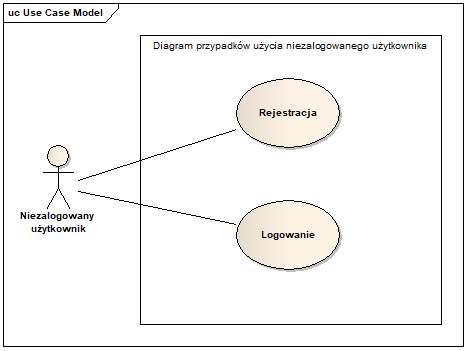
\includegraphics[width=0.6\textwidth]{./graf/Przypadki_uzycia_niezalogowany.png}
\caption{Diagram przypadków użycia niezalogowanego użytkownika.}
\label{fig:1}
\end{figure}

\begin{figure}
\centering
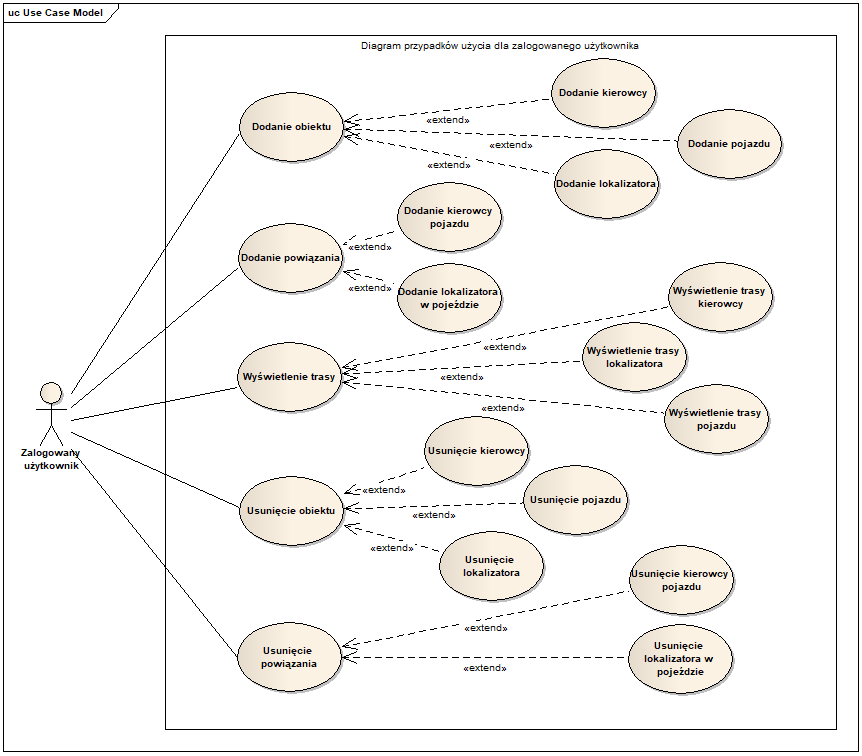
\includegraphics[width=1\textwidth]{./graf/Przypadki_uzycia_zalogowany.png}
\caption{Diagram przypadków użycia zalogowanego użytkownika.}
\label{fig:2}
\end{figure}

\paragraph{}
Aby przystąpić do tworzenia aplikacji, należało przygotować odpowiednie narzędzia. W pierwszej kolejności zakupiono lokalizator TK108 oraz kartę SIM, aby możliwe było uruchomienie i skonfigurowanie urządzenia. Kolejnym etapem było zainstalowanie niezbędnego oprogramowania do edycji kodu źródłowego aplikacji. Do części funkcjonalnej został wykorzystany Intellij Idea wydawcy JetBrains. Ten program jest zaawansowanym, wieloplatformowym środowiskiem programistycznym, posiadającym dużą ilość wbudowanych narzędzi, jak również obsługującym wiele bibliotek i platform programistycznych, takich jak Spring Boot. Hibernate oraz JPA również są wspierane przez Intellij. Są to narzędzia, które potrafią powiązać kod aplikacji z bazą danych, co znacznie uprości rozwijanie programu. W kontekście bazy danych, potrzebne było oprogramowanie, które będzie w stanie obsługiwać zapytania kierowane do bazy danych - na początku do stworzenia bazy, poszczególnych tabel, a w przyszłości do eliminiowania ewentualnych błędów oraz do testowania aplikacji. Przechodząc do interfejsu użytkownika, a zatem do kodu w języku TypeScript z zastosowaniem biblioteki React, wybrano Microsoft Visual Studio Code, który jest powszechnie używany przez programistóW w tym celu, ze względu na odpowiednie wsparcie języków i bibliotek typowych do tworzenia wizualnej części aplikacji. Ostatnim elementem jest narzędzie do systemu kontroli wersji. Dzięki temu postępy w pracy będą zabezpieczone. Nie mniej jednak, to nie jedyny atut. W przypadku błędów aplikacji spowodowanych zmianami w kodzie źródłowym, zlokalizowanie ich przyczyny będzie znacznie ułatwione. Wybrano system Git, gdyż jest on najpopularniejszą opcją, a co za tym idzie, jest obsługiwany przez niemal każde oprogramowanie programistyczne, lecz to nie wszystko. Należy również dokonać wyboru platformy hostingowej, która będzie przechowywała repozytorium Git. W tym celu skorzystano z GitHuba, będącego jedną z najbardziej powszechnych opcji. Jest on także wspierany przez większość środowisk programistycznych. 

%\begin{itemize}
%\item wymagania funkcjonalne i niefunkcjonalne
%\item przypadki użycia (diagramy UML) -- dla prac, w których mają zastosowanie
%\item opis narzędzi, metod eksperymentalnych, metod modelowania itp.
%\item metodyka pracy nad projektowaniem i implementacją -- dla prac, w których ma to zastosowanie
%\end{itemize}
 % Wymagania i narzędzia

% TODO
\chapter{Specyfikacja zewnętrzna}
\label{ch:04}

\paragraph{}
Specyfikacja zewnętrzna opisuje interakcje użytkownika z systemem, jak również jego wygląd i sposób obsługi. Niniejszy rozdział zawiera także informacje na temat wymagań sprzętowych, które należy spełnić, aby aplikacja działała poprawnie.

\section{Wymagania sprzętowe i programowe}
\paragraph{}
Aplikacja do działania potrzebuje serwera - komputera, na którym skompilowany z kodu źródłowego program, jak również baza danych, będą uruchomione. Serwer musi posiadać dostęp do internetu oraz jego adres musi być publicznie dostępny. Dzięki temu ma on możliwość obsługiwania żądań HTTP wysyłanych przez użytkowników.

\paragraph{}
W przypadku działającego serwera, można do użytkowania aplikacji. W celu uzyskania do niej dostępu, użytkownik musi mieć zainstalowaną przeglądarkę na urządzeniu (np. komputerze stacjonarnym, laptopie, tablecie czy smartfonie) oraz połączenia z internetem. Po spełnieniu powyższych wymagań, w pasek adresu URL w przeglądarce należy wpisać adres serwera oraz port, na którym uruchomiona jest aplikacja. Można również uprościć użytkownikom uruchomienie aplikacji poprzez uruchomienie serwera na konkretnej domenie DNS, którą wystarczy wpisać w przeglądarce, natomiast nie zostało to zaimplementowane w trakcie procesu tworzenia systemu.

\section{Kategorie użytkowników}
\paragraph{}
Wyróżniamy dwa rodzaje użytkowników: 
\begin{itemize}
	\item niezalogowany użytkownik
	\item zalogowany użytkownik
\end{itemize}

\paragraph{}
Z niezalogowanym użytkownikiem mamy do czynienia wówczas, gdy nastąpi włączenie aplikacji lub po wylogowaniu się ze swojego konta podczas użytkowania. Funkcje, które ma on do dyspozycji, są mocno ograniczone. Użytkownik ma wtedy dostęp do:
\begin{itemize}
	\item strony głównej - tylko wyświetla tekst 
	\item formularza rejestracji - pozwala utworzyć konto użytkownika
	\item formularza logowania - umożliwia zalogowanie się na istniejące w systemie konto
\end{itemize}

\paragraph{}
Zalogowany użytkownik uzyskuje dostęp do właściwych funkcji systemu, dzięki którym może zarządzać lokalizatorami, jak również kierowcami i pojazdami.

\section{Sposób obsługi}
\paragraph{}
Po włączeniu aplikacji ukazuje się strona główna. Widoczny na niej tekst zachęca do skorzystania z wszystkich funkcji systemu. Jej wygląd jest widoczny na rys. \ref{fig:home_page}. Na górze strony znajduje się pasek nawigacji, który towarzyszy użytkownikowi przez cały czas użytkowania programu, lecz różni się w zależności od tego, czy użytkownik jest niezalogowany (pasek wtedy przybiera formę jak na rys. \ref{fig:home_page}, czy zalogowany (w tym przypadku pasek wygląda jak na rys.\ref{fig:user_tab}). Po kliknięciu w poszczególną opcję na pasku, odpowiadająca jej zakładka jest otwierana. Aby przejść do formularzy logowania i rejestracji, należy wybrać opcję "Zaloguj się".

\begin{figure}
	\centering
	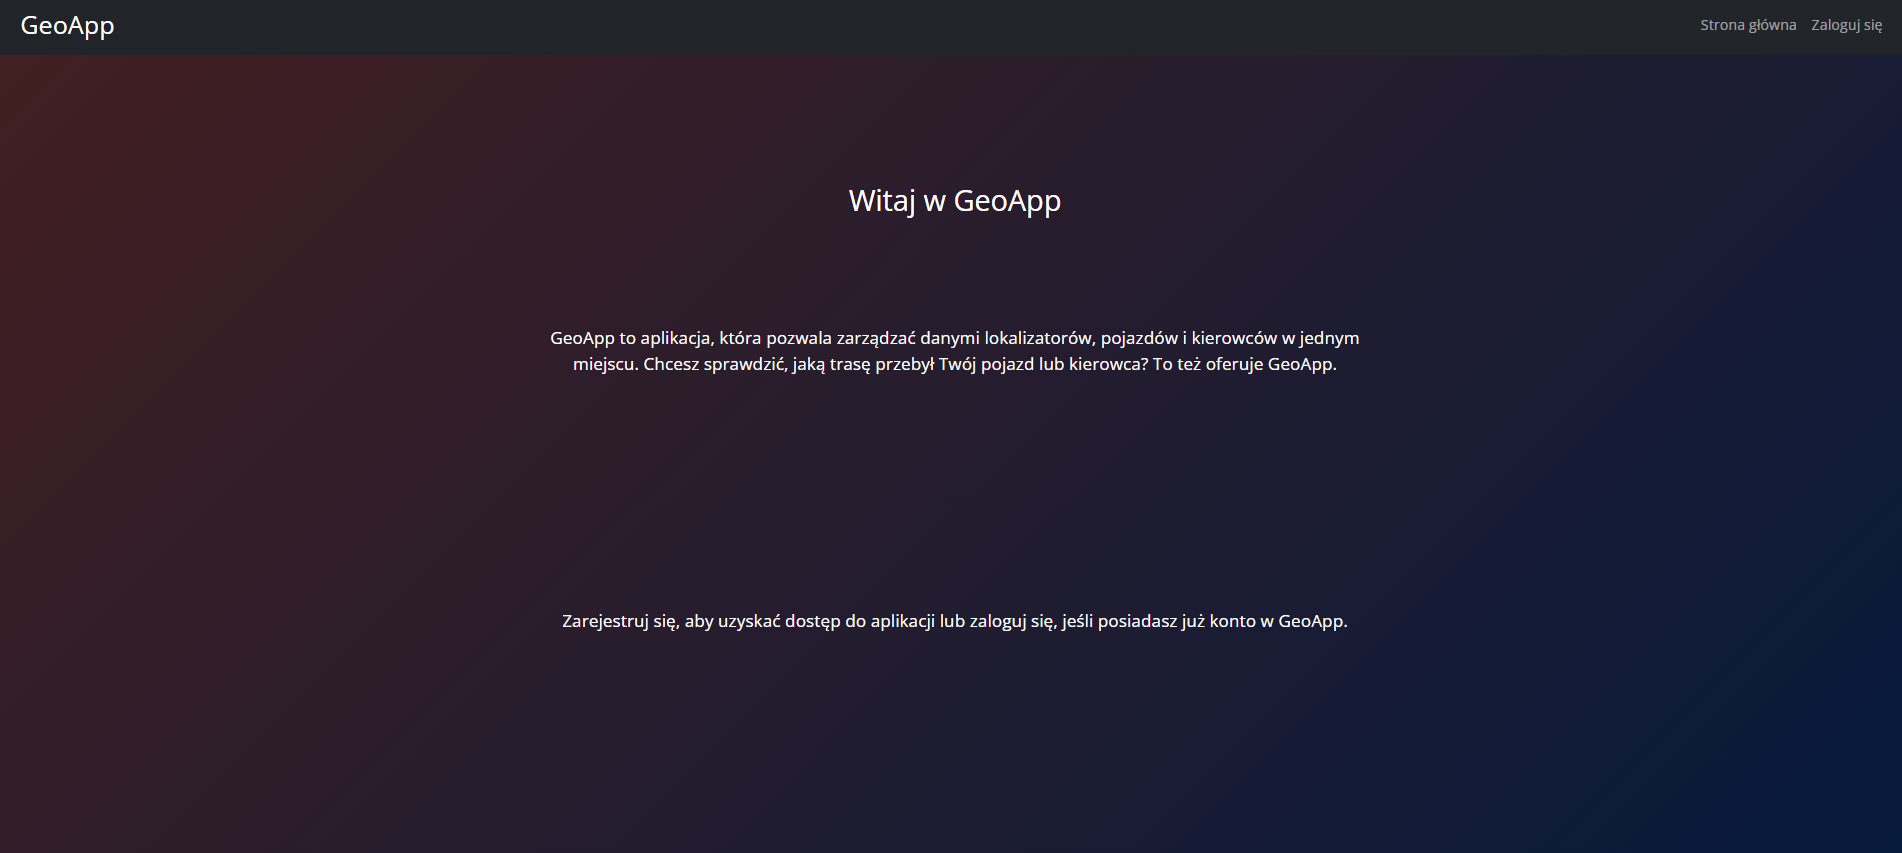
\includegraphics[width=1\textwidth]{./graf/home_page.png}
	\caption{Zrzut ekranu przedstawiający stronę główną.}
	\label{fig:home_page}
\end{figure}

\paragraph{}
W pierwszej kolejności ukazuje się formularz logowania (rys. \ref{fig:login_form}). Jest to celowy zabieg, ponieważ użytkownik, po założeniu konta, z każdym kolejnym uruchomieniem aplikacji będzie się logował. Wynika z tego, iż liczba logowań będzie wyższa niż liczba rejestracji, a zatem będzie to częstsza operacja wykonywana przez użytkowników. W celu otwarcia formularza rejestracji, należy kliknąć w tekst w lewym dolnym rogu formularza logowania. Jego treść brzmi: „Nie masz jeszcze konta? Zarejestruj się” - rys. \ref{fig:login_form}. Jest to link, który umożliwia zmianę formularza z opcji do zalogowania się, na opcję do utworzenia konta. Aby stworzyć konto użytkownika, należy wpisać adres email, z którym będzie owe konto powiązane. Kolejnym etapem jest ustalenie hasła, którym następnie wypełnia się drugie pole. W celach bezpieczeństwa, hasło powinno być trudne do rozszyfrowania przez innych ludzi. Niemniej jednak, nie ma możliwości odzyskania zapomnianego hasła, o czym warto pamiętać podczas korzystania z aplikacji. Aby dokończyć proces tworzenia konta, należy nacisnąć niebieski przycisk w prawym dolnym rogu. Widok formularza rejestracji znajduje się na rys. \ref{fig:register_form}.

\begin{figure}
	\centering
	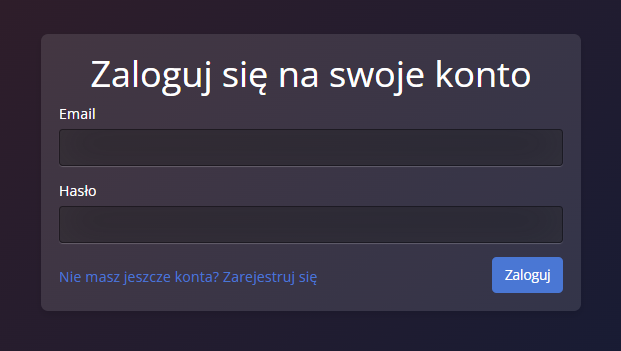
\includegraphics[width=0.6\textwidth]{./graf/login_form.png}
	\caption{Zrzut ekranu przedstawiający formularz logowania.}
	\label{fig:login_form}
\end{figure}

\begin{figure}
	\centering
	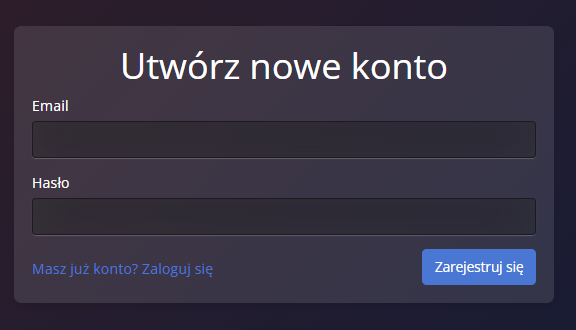
\includegraphics[width=0.6\textwidth]{./graf/register_form.png}
	\caption{Zrzut ekranu przedstawiający formularz rejestracji.}
	\label{fig:register_form}
\end{figure}

\paragraph{}
Do formularza logowania można dostać się na dwa sposoby. Jeden został wymieniony powyżej, drugim jest kliknięcie w tekst znajdujący się w lewym dolnym narożniku formularza rejestracji, brzmiący: „Masz już konto? Zaloguj się”. Dzięki temu w prosty sposób można przejść do zalogowania się, bezpośrednio po stworzeniu konta. Formularz logowania zawiera dwa pola, jedno służy do wpisania adresu email, z którym powiązane jest konto. W drugie pole należy wpisać hasło, które zostało ustalone podczas rejestracji. Zamiast znaków wpisywanych w to pole, pojawiają się kropki. Jest to mechanizm służący podniesieniu bezpieczeństwa, aby żadna dodatkowa osoba będąca w bliskiej okolicy użytkownika nie była w stanie przeczytać hasła, które jest wprowadzane. Po wypełnieniu obydwu pól wystarczy kliknąć niebieski przycisk pod formularzem.

\paragraph{}
W przypadku poprawnego wprowadzenia emailu oraz hasła, na ekranie ukazuje się panel użytkownika (rys.\ref{fig:user_tab}). Służy on przede wszystkim do dodawania powiązań między kierowcami, pojazdami i lokalizatorami, natomiast w pierwszej kolejności trzeba dodać poszczególne obiekty, jakimi są kierowca, pojazd czy lokalizator. Niemniej jednak, założono, że w trakcie używania aplikacji, użytkownicy nie często będą dodawać np. nowe pojazdy, stąd pierwszą zakładką, jaka pokazuje się po zalogowaniu, jest panel użytkownika. 

\begin{figure}
	\centering
	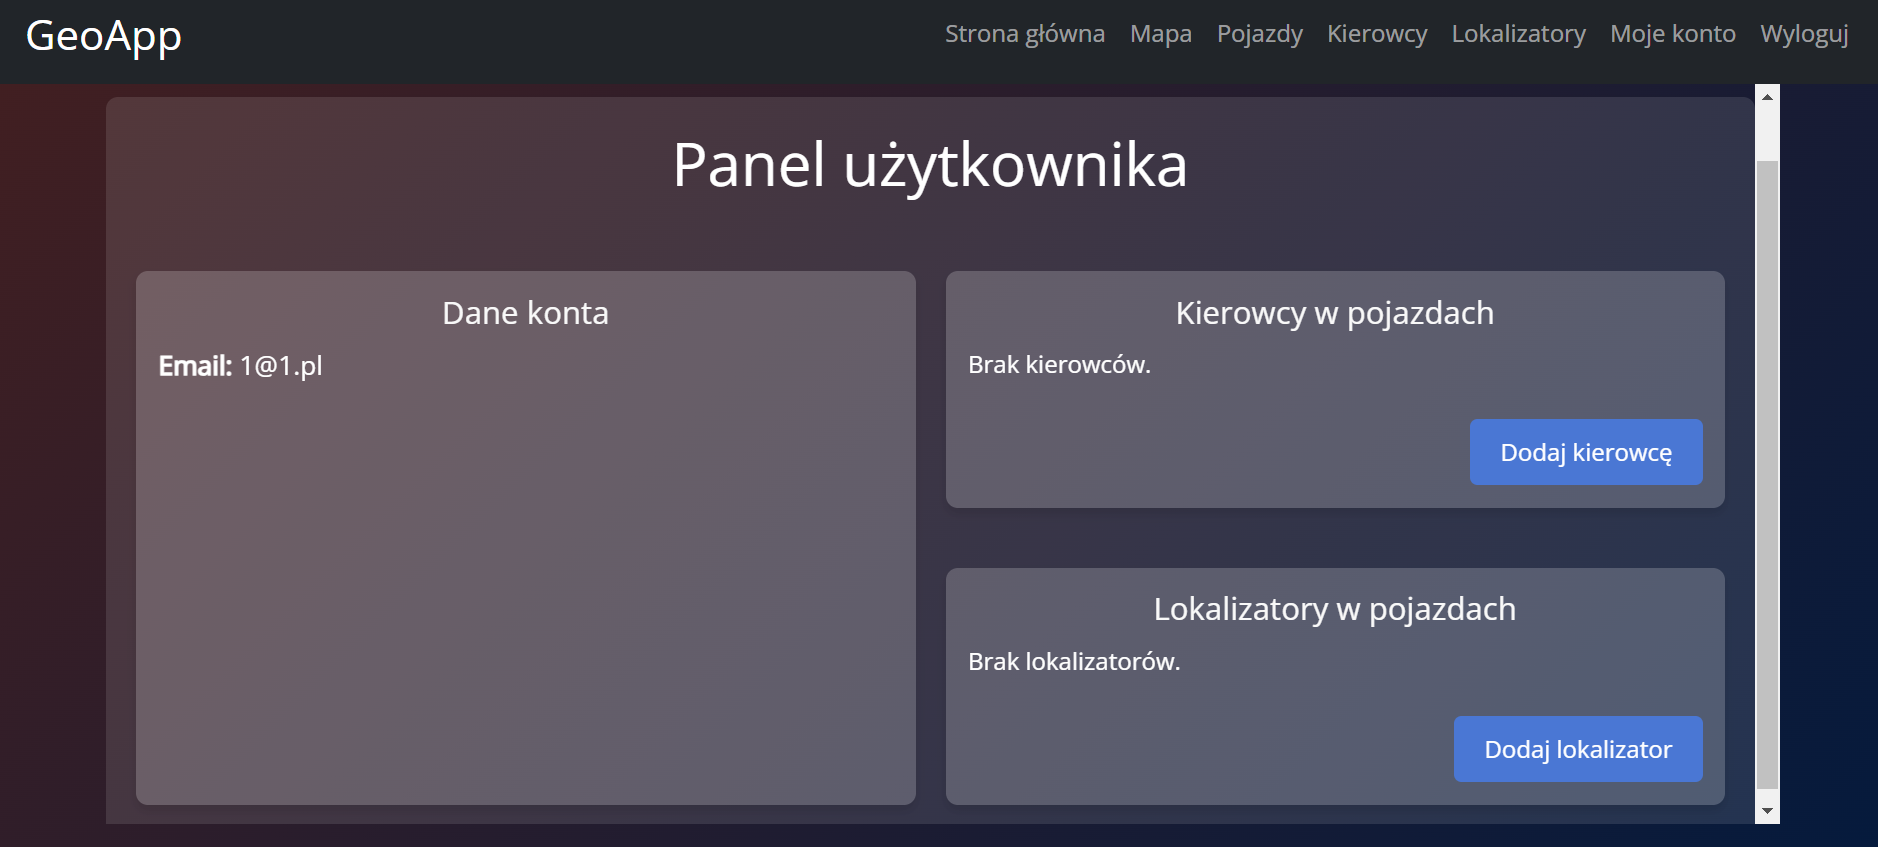
\includegraphics[width=0.6\textwidth]{./graf/user_tab.png}
	\caption{Zrzut ekranu przedstawiający zakładkę Moje konto.}
	\label{fig:user_tab}
\end{figure}


\paragraph{}
Aby dodać kierowcę, w pierwszej kolejności należy przejść do zakładki nazwanej „Kierowcy”. Podstawowym elementem tej części aplikacji jest lista kierowców. W przypadku gdy lista jest pusta, wyświetlany jest tekst „Brak kierowców.”, widoczny na rys. \ref{fig:driver_tab}. Pod listą lub napisem świadczącym o pustej liście znajduje się przycisk służący do dodania nowego kierowcy do listy. Po naciśnięciu przycisku otworzy się formularz - jego wygląd jest dostępny na rys. \ref{fig:add_driver}. Należy wypełnić jego pola, którymi są imię oraz nazwisko kierowcy. Przycisk oznaczony napisem „Dodaj kierowcę” pozwala dokończyć proces i zapisać wprowadzone dane w systemie. Formularz zostanie zamknięty, a na liście pojawi się nowa pozycja - przykład widoku z przykładowym kierowcą przedstawia rys. \ref{fig:driver_tab_2}. W przypadku kliknięcia czerwonego przycisku „Anuluj”, proces dodawania kierowcy zostanie wycofany, a aplikacja wróci do widoku zakładki z listą kierowców. Będąc tej w zakładce, użytkownik ma również możliwość usunięcia wybranego kierowcy. Służy do tego przycisk „Usuń”, znajdujący się po prawej stronie od każdej pozycji na liście.

\begin{figure}
	\centering
	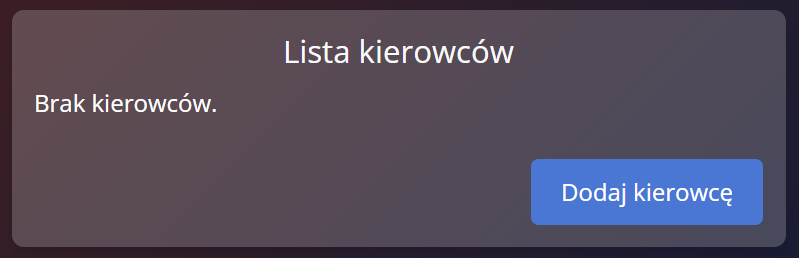
\includegraphics[width=0.6\textwidth]{./graf/driver_tab.png}
	\caption{Zrzut ekranu przedstawiający zakładkę Kierowcy.}
	\label{fig:driver_tab}
\end{figure}

\begin{figure}
	\centering
	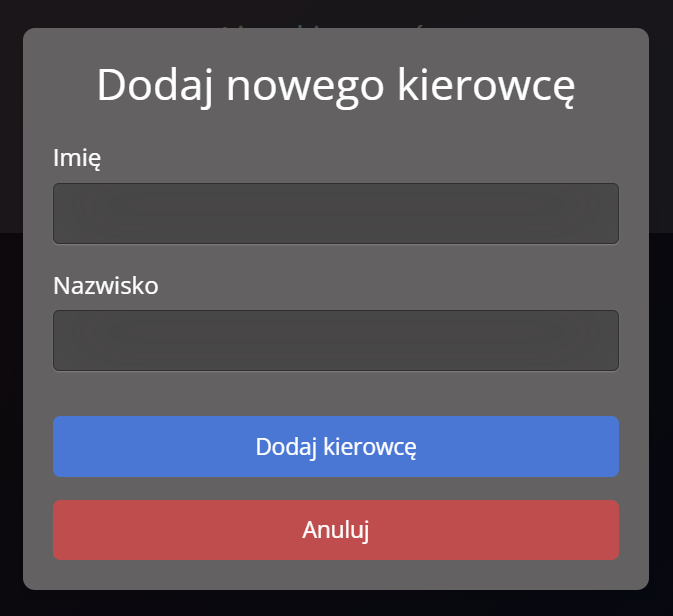
\includegraphics[width=0.6\textwidth]{./graf/add_driver.png}
	\caption{Zrzut ekranu przedstawiający formularz dodawania kierowcy.}
	\label{fig:add_driver}
\end{figure}

\begin{figure}
	\centering
	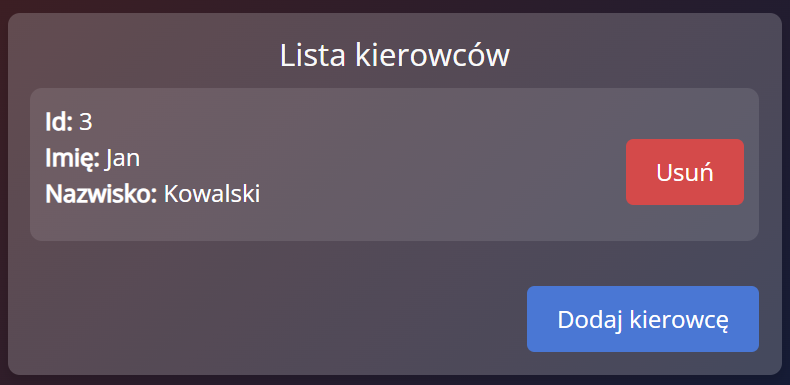
\includegraphics[width=0.6\textwidth]{./graf/driver_tab_2.png}
	\caption{Zrzut ekranu przedstawiający zakładkę Kierowcy z jednym kierowcą na liście.}
	\label{fig:driver_tab_2}
\end{figure}

\paragraph{}
Zakładką o analogicznym działaniu jest zakładka „Pojazdy”. Posiada listę samochodów zalogowanego użytkownika oraz przycisk pozwalający dodać do niej nową pozycję - wygląd z pustą listą znajduje się na rys. \ref{fig:vehicle_tab}. Formularz w tym przypadku posiada cztery pola: marka, model, tablica rejestracyjna oraz VIN. Pierwsze dwa służą przede wszystkim zwiększeniu przejrzystości listy dla użytkownika, natomiast trzecie i czwarte pole umożliwiają rozróżnienie poszczególnych samochodów, podczas gdy są one tej samej marki oraz tego samego modelu. Rys. \ref{fig:add_vehicle} przedstawia formularz dodawania pojazdu. Usuwanie elementów z listy jest dostępne również za pomocą przycisku znajdującego się po prawej stronie od każdego pojazdu.

\begin{figure}
	\centering
	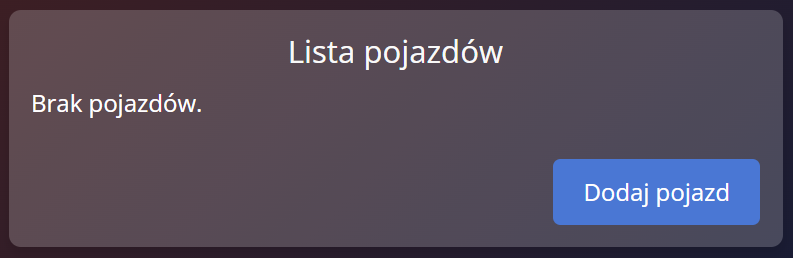
\includegraphics[width=0.6\textwidth]{./graf/vehicle_tab.png}
	\caption{Zrzut ekranu przedstawiający zakładkę Pojazdy.}
	\label{fig:vehicle_tab}
\end{figure}

\begin{figure}
	\centering
	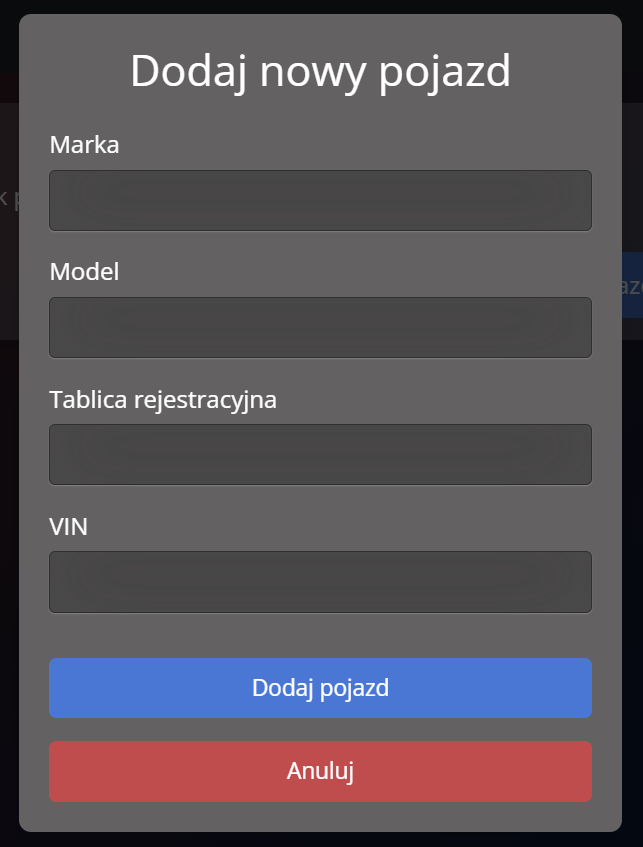
\includegraphics[width=0.6\textwidth]{./graf/add_vehicle.png}
	\caption{Zrzut ekranu przedstawiający formularz dodawania pojazdu.}
	\label{fig:add_vehicle}
\end{figure}

\paragraph{}
„Lokalizatory” to trzecia zakładka o podobnej zasadzie działania. Zrzut ekranu z jej wyglądem jest dostępny na rys. \ref{fig:tracker_tab}. Lista zawiera lokalizatory dodane przez użytkownika. Po kliknięciu w przycisk zatytułowany „Dodaj lokalizator”, otworzy się formularz, tym razem posiadający trzy pola do wypełnienia (rys.\ref{fig:add_tracker}). Nazwa jest dowolna, ma na celu ułatwić użytkownikowi znalezienie pożądanego lokalizatora na liście, numer seryjny jest polem identyfikacyjnym, które jest niepowtarzalne dla każdego urządzenia, natomiast w pole typ należy wpisać model urządzenia. W tym formularzu pojawia się również dodatkowy przycisk z napisem "Instrukcja - konfiguracja lokalizatora". Otwiera on dodatkowe okno z punktami, które trzeba wykonać, aby skonfigurować urządzenie do działania z aplikacją (rys. \ref{fig:help_dialog}). Można je zamknąć przyciskiem "Anuluj". Usuwanie odbywa się za pomocą przycisku „Usuń”, widocznego na rys. \ref{fig:tracker_tab}.

\begin{figure}
	\centering
	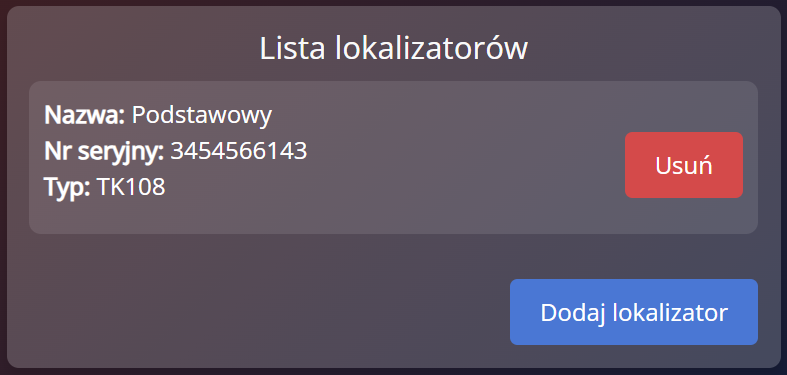
\includegraphics[width=0.6\textwidth]{./graf/tracker_tab.png}
	\caption{Zrzut ekranu przedstawiający zakładkę Lokalizatory.}
	\label{fig:tracker_tab}
\end{figure}

\begin{figure}
	\centering
	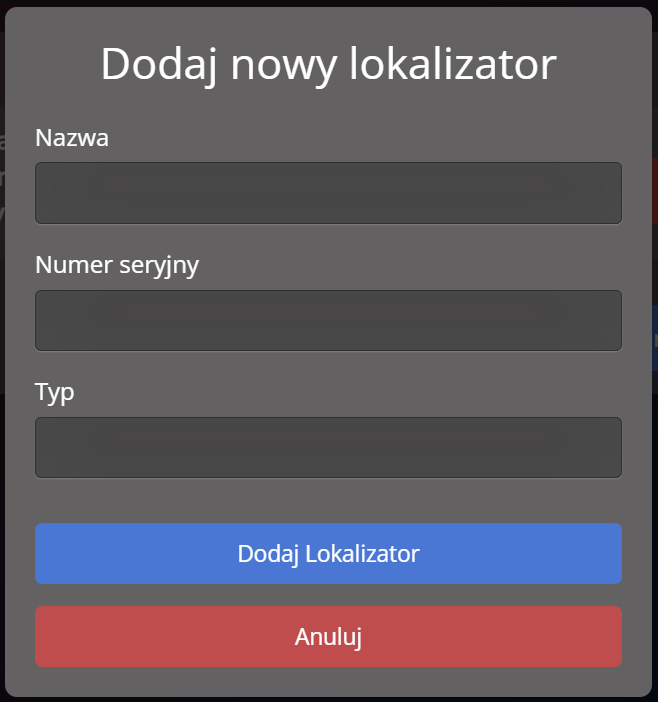
\includegraphics[width=0.6\textwidth]{./graf/add_tracker.png}
	\caption{Zrzut ekranu przedstawiający formularz dodawania lokalizatora.}
	\label{fig:add_tracker}
\end{figure}

\begin{figure}
	\centering
	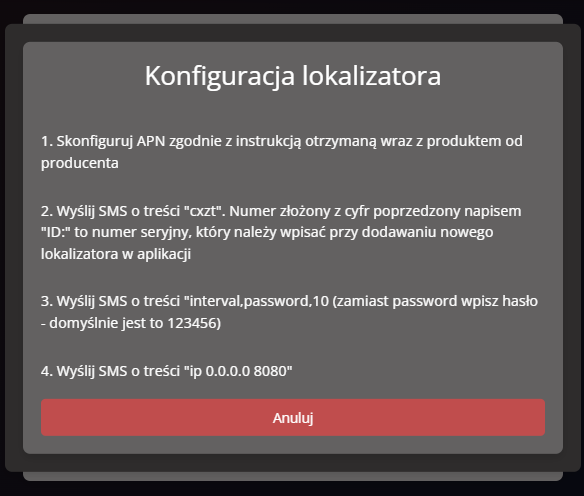
\includegraphics[width=0.6\textwidth]{./graf/help_dialog.png}
	\caption{Zrzut ekranu przedstawiający formularz dodawania lokalizatora.}
	\label{fig:help_dialog}
\end{figure}

\paragraph{}
Po dodaniu kierowców, pojazdów i lokalizatorów można przejść do tworzenia powiązań między nimi. W tym celu należy otworzyć zakładkę „Moje konto”, która przedstawia panel użytkownika. Aplikacja pozwala na stworzenie dwóch rodzajów powiązań:

\begin{itemize}
	\item kierowca pojazdu
	\item lokalizator w pojeździe
\end{itemize}

\paragraph{}
Kierowcy pojazdów, będący jednocześnie tytułem pierwszej listy w panelu użytkownika, definiują w jakim okresie czasu dany kierowca korzysta z danego pojazdu. Będzie to miało szczególne znaczenie podczas wyświetlania tras przebytych przez poszczególną osobę. W celu dodania powiązania, należy kliknąć przycisk „Dodaj kierowcę” (\ref{fig:user_tab}). Aplikacja wyświetli formularz składający się z czterech pól (rys. \ref{fig:add_driver_vehicle}). Pierwsze dwa są polami rozwijanymi, elementami pierwszego będą wszystkie pojazdy użytkownika, natomiast w drugim znajdować się będą jego kierowcy. Kolejne dwa pola to początek i koniec okresu użytkowania wybranego samochodu przez wybraną osobę. W celu wyznaczenia dat należy wybrać odpowiedni dzień z wyświetlonego kalendarza. Aby dokończyć proces tworzenia powiązania, należy kliknąć przycisk z napisem „Dodaj powiązanie”. Powiązanie zostanie zapisane do bazy danych i wyświetli się jako nowy element listy. Przycisk „Anuluj” czyści pola formularza jednocześnie go zamykając.

\begin{figure}
	\centering
	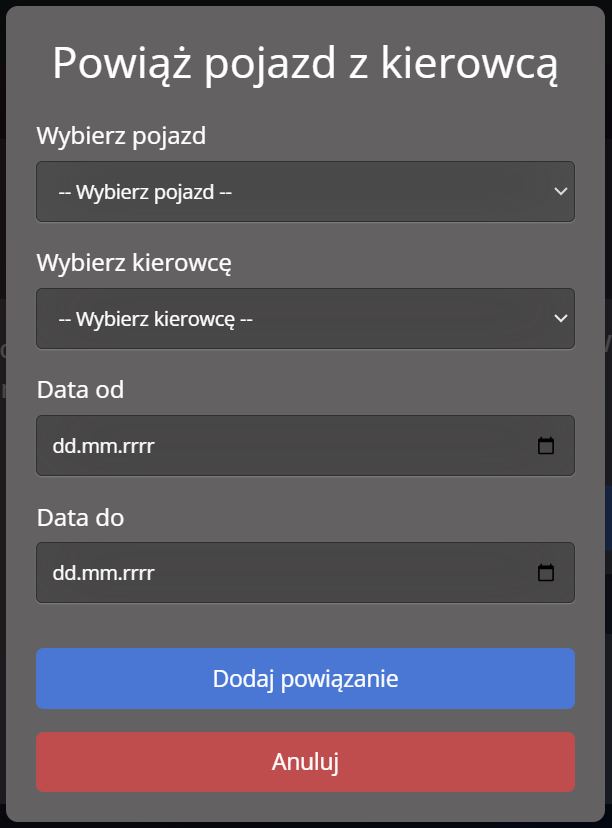
\includegraphics[width=0.6\textwidth]{./graf/add_driver_vehicle.png}
	\caption{Zrzut ekranu przedstawiający formularz dodawania powiązania kierowcy z pojazdem.}
	\label{fig:add_driver_vehicle}
\end{figure}


\paragraph{}
Drugą opcją powiązań są lokalizatory w pojazdach. Ich lista znajduje się pod listą kierowców pojazdów. Podobnie jak w przypadku pierwszego powiązania, formularz, który pozwala na dodanie nowego elementu od listy, ma cztery pola. Pierwsze pole jest niezmienione, co można zobaczyć na rys. \ref{fig:add_tracker_vehicle}. Jest to spowodowane faktem, iż to powiązanie również wykorzystuje pojazdy, zatem można w tym miejscu dokonać wyboru samochodu. Drugie pole uległo zmianie, jest to rozwijana lista lokalizatorów, z których należy wybrać jeden, który w danym okresie użytkownik planuje umieścić w pojeździe. Okres powiązania definiują kolejne dwa pola formularza, które również nie różnią się od pól wypełnianych podczas dodawania powiązania kierowcy z pojazdem. Przyciski oraz ich działanie jest także analogiczne do powyżej opisanego powiązania.

\begin{figure}
	\centering
	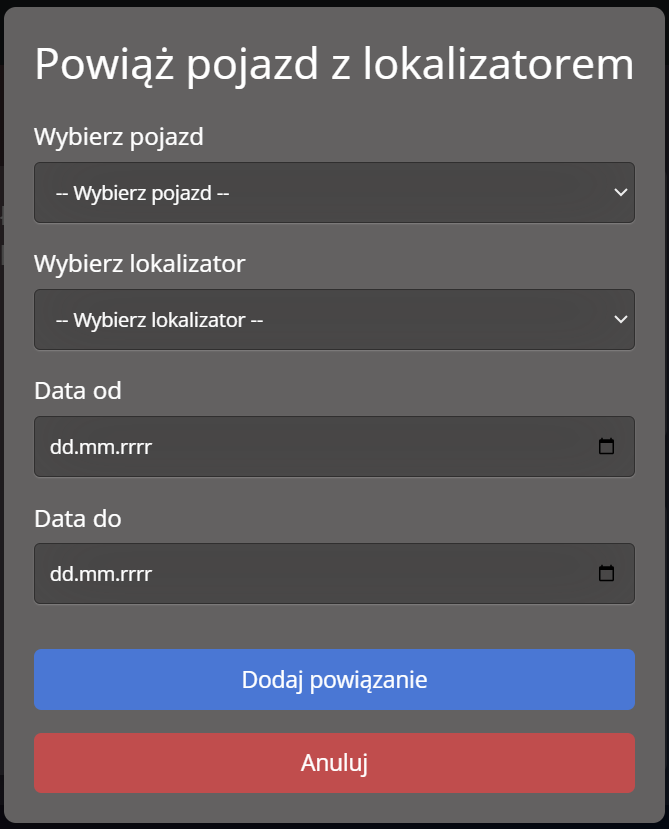
\includegraphics[width=0.6\textwidth]{./graf/add_tracker_vehicle.png}
	\caption{Zrzut ekranu przedstawiający formularz dodawania powiązania lokalizatora z pojazdem.}
	\label{fig:add_tracker_vehicle}
\end{figure}

\paragraph{}
Usuwania powiązań dokonuje się w identyczny sposób, w jaki zostało opisane usuwanie pojedynczych obiektów. Niemniej jednak, ważnym aspektem usuwania kierowców, pojazdów i lokalizatorów jest fakt, iż w przypadku uczestnictwa danego obiektu w jakimkolwiek powiązaniu, niedozwolone jest jego usunięcie. Pierwszym krokiem jest wtedy wyeliminowanie powiązania, z którym związany jest wybrany przez użytkownika np. kierowca, a następnie przeprowadzenie procesu usunięcia kierowcy.

\begin{figure}
	\centering
	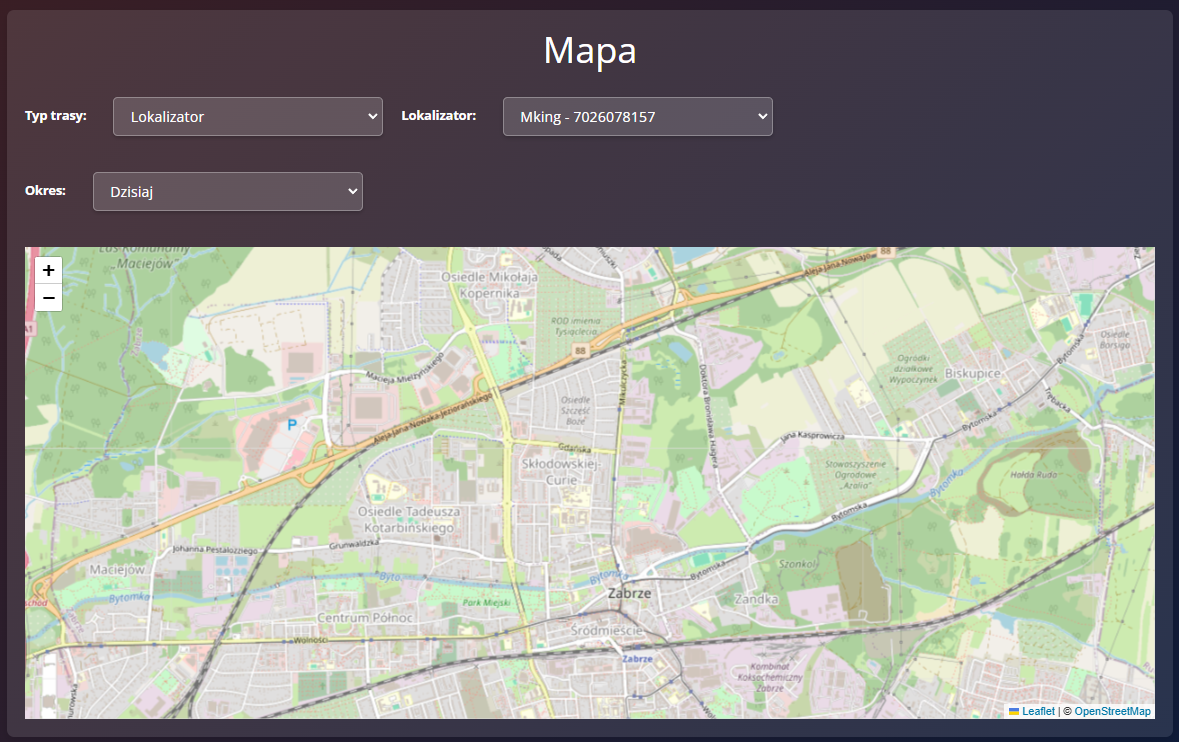
\includegraphics[width=0.6\textwidth]{./graf/map_tab.png}
	\caption{Zrzut ekranu przedstawiający zakładkę Mapa.}
	\label{fig:map_tab}
\end{figure}

\paragraph{}
Zakładka pod tytułem „Mapa” pozwala na wyświetlenie trasy z danego okresu czasu. Po jej otwarciu oczom użytkownika ukazuje się widok z rys. \ref{fig:map_tab}. Mapę można oddalać oraz przybliżać, korzystając z kółka myszy, a także przesuwać, poruszając myszą przy wciśniętym lewym przycisku. Pierwszą trasą, która wyświetla się po otwarciu zakładki jest trasa pierwszego z listy lokalizatora z bieżącego dnia, oczywiście w przypadku gdy ten lokalizator wysyłał dane na serwer tego dnia, to znaczy nie był wyłączony, rozładowany oraz został poprawnie skonfigurowany. Rozwijana lista nazwana "Lokalizator" pozwala wybrać konkretne urządzenie, którego trasę chcemy zobaczyć na mapie (rys. \ref{fig:/map_tracker}). Aby zmienić trasę na kierowcę lub pojazd, należy rozwinąć pole opisane jako "Typ trasy". Można wybrać wtedy opcję z listy, co widać na rys. \ref{fig:map_type}. W zależności od wybranego typu, rozwijana lista oznaczona słowem "Lokalizator" zmienia się w listę wyboru kierowcy lub pojazdu. Ostatnią opcją do wyboru jest "Okres", czyli dzień lub zakres dat, z którego chcemy wyświetlić trasę. Zgodnie z tym, co znajduje się na rys. \ref{fig:map_period}, można wybrać jedną z paru opcji domyślnych lub opcję "Niestandardowy", której kliknięcie skutkuje pojawieniem się dodatkowych dwóch pól (rys. \ref{fig:map_period}), w celu określenia daty początkowej i końcowej okresu do wyświetlenia trasy. Przykład ukazujący wygląd losowej trasy przedstawia rys. \ref{fig:map_route}.

\begin{figure}
	\centering
	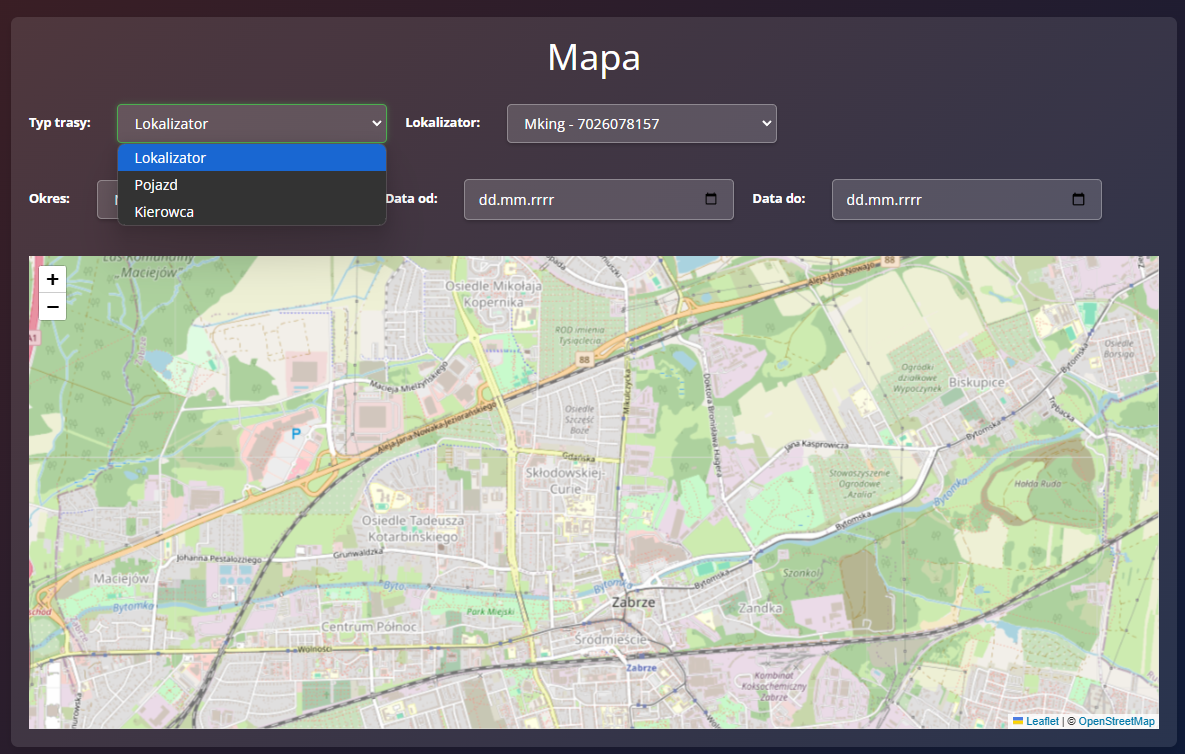
\includegraphics[width=1\textwidth]{./graf/map_type.png}
	\caption{Zrzut ekranu przedstawiający formularz dodawania trasy kierowcy.}
	\label{fig:map_type}
\end{figure}

\begin{figure}
	\centering
	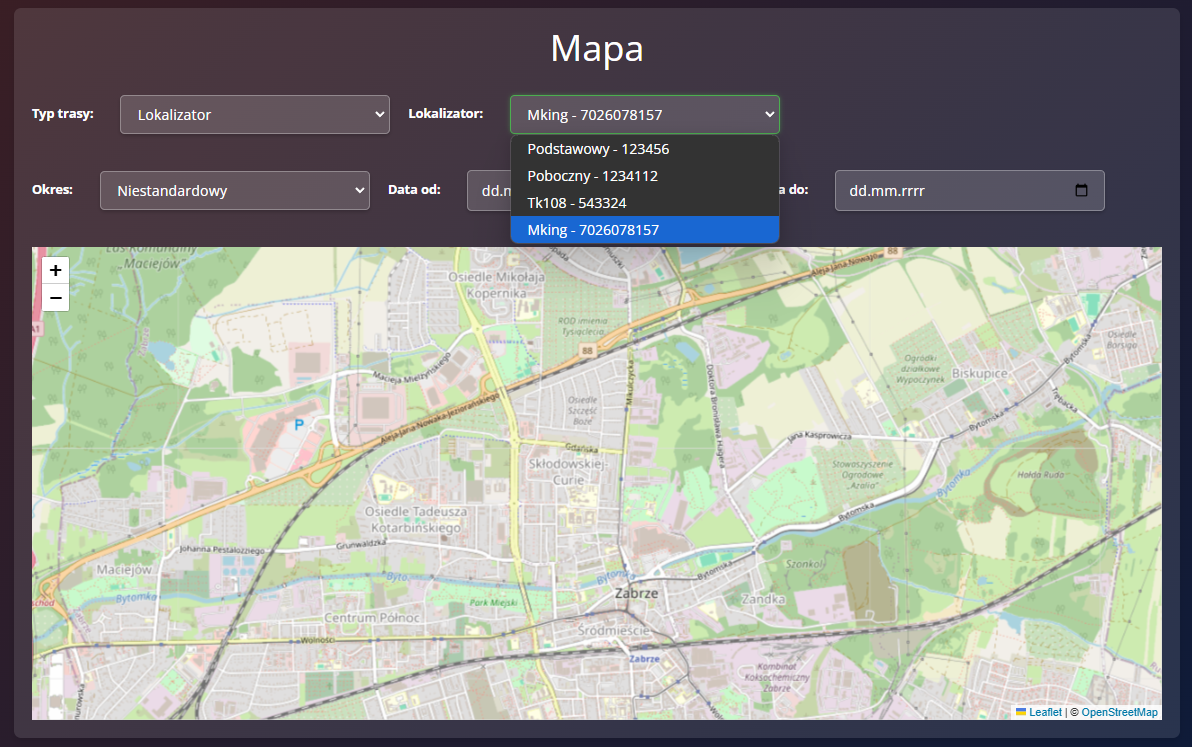
\includegraphics[width=1\textwidth]{./graf/map_tracker.png}
	\caption{Zrzut ekranu przedstawiający formularz dodawania trasy pojazdu.}
	\label{fig:/map_tracker}
\end{figure}

\begin{figure}
	\centering
	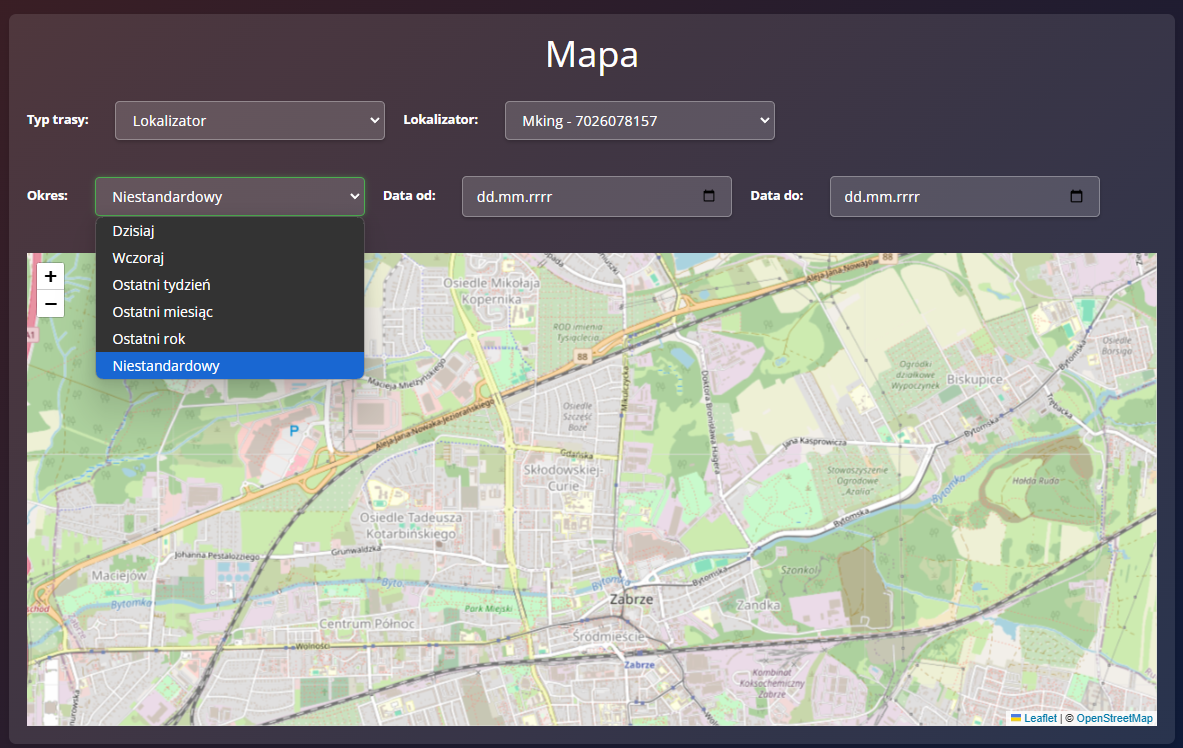
\includegraphics[width=1\textwidth]{./graf/map_period.png}
	\caption{Zrzut ekranu przedstawiający mapę z jedną trasą.}
	\label{fig:map_period}
\end{figure}

\begin{figure}
	\centering
	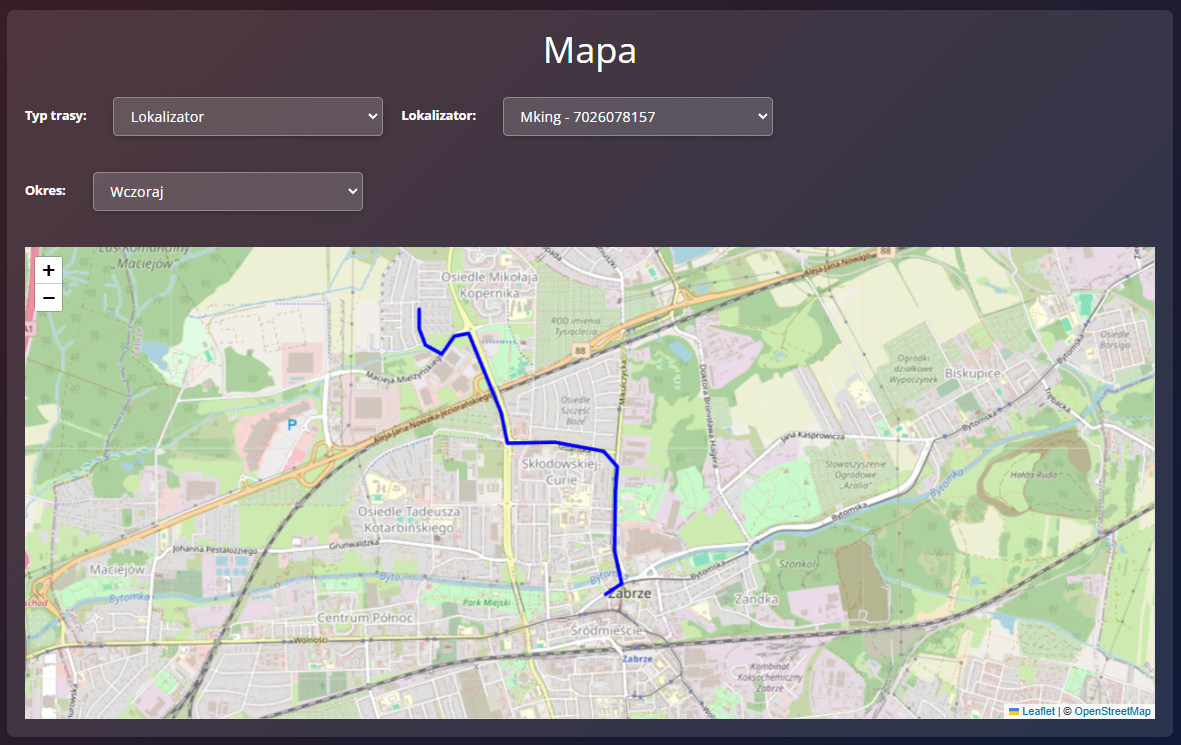
\includegraphics[width=1\textwidth]{./graf/map_route.png}
	\caption{Zrzut ekranu przedstawiający mapę z jedną trasą.}
	\label{fig:map_route}
\end{figure}


\paragraph{}
Na pasku nawigacyjnym zalogowanego użytkownika widnieje jeszcze jedna zakładka - „Wyloguj się” (rys. \ref{fig:user_tab}). Jest to tak naprawdę przycisk umożliwiający wylogowanie się z konta uzytkownika. Po jego kliknięciu, aplikacja nas wylogowuje i przenosi do strony głównej. Pojawia się wtedy pasek nawigacji widoczny na rys. \ref{fig:home_page}, co sprawia, iż w celu dostępu do funkcji zalogowanego użytkownika, należy ponownie się zalogować zgodnie z wyżej opisanymi krokami.

 % [Właściwy dla kierunku -- np. Specyfikacja zewnętrzna]

% TODO
\chapter{Specyfikacja wewnętrzna}
\label{ch:05}

\paragraph{}
Specyfikacja wewnętrzna jest ważnym elementem dokumentacji technicznej. Pozwala na zrozumienie funkcjonowania aplikacji, dzięki zawartym opisom struktur danych, architektury systemu, jak również tłumaczeniom kodu źródłowego, popartym jego fragmentami.

\section{Przedstawienie architektury systemu}
\paragraph{}
Podczas pisania kodu źródłowego kierowano się podejściem database-first, co oznacza rozpoczęcie prac od zaprojektowania bazy danych. Pierwszym krokiem było przygotowanie schematu, który znajduje się na rys. \ref{fig:database}, który jest opisanyw następnym podrozdziale. W oparciu o schemat utworzono bazę danych, a następnie odpowiadające tabelom klasy encji w języku Java. Po zakończeniu poprzednich kroków, rozpoczęto pisanie kodu interfejsu oraz tego odpowiadającego za logikę aplikacji. 

\paragraph{}
Aplikacja podzielona jest na trzy warstwy, co obrazuje schemat wdrożenia (rys. \ref{deployment_diagram}). Aplikacja na urządzeniu użytkownika reprezentuje frontend, czyli część związaną z interfejsem. Serwer aplikacji oznacza backend - część funkcjonalną. Dwie opisane wartswy programu komunikują sę ze sobą przy użyciu ządań HTTP. Backend komunikuje się również z bazą danych - trzecią częścią aplikacji - z wykorzystaniem JPA oraz Hibernate. Ostatnim elementem schematu jest lokalizator, nie należący do żadnej z warstw aplikacji, natomiast jest on ważnym elemnetem podczas działania systemu i komunikuje się z częścią funkcjonalną za pomocą protokołu TCP.

\begin{figure}
	\centering
	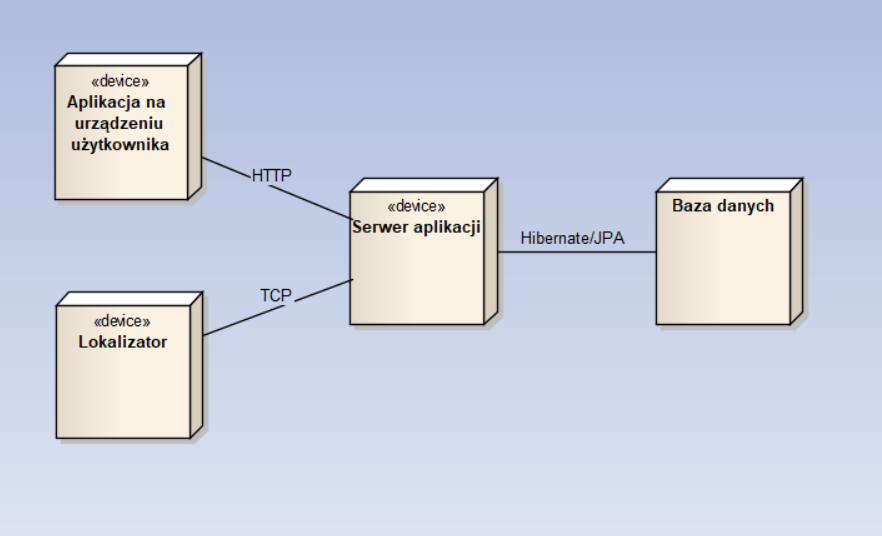
\includegraphics[width=1\textwidth]{./graf/deployment_diagram.png}
	\caption{Diagram wdrożenia.}
	\label{deployment_diagram}
\end{figure}

\paragraph{}
Widok użytkownika (frontend) napisany został w języku TypeScript, bazuje na komponentach biblioteki React. Podłoże aplikacji (backend) jest oparte na języku Java. Znanym wzorcem projektowym jest MVC (ang. Model View Controller), co przetłumaczone na język polski brzmi: model, widok, kontroler. Model to cześć odpowiadająca za przechowywanie danych. Widok to część dostępna dla użytkownika aplikacji, natomiast kontroler wykonuje operacje i jest odpowiedzialny za logikę programu. Do stworzenia programu wykorzystano architekturę warstwową, która bazuje na MVC oraz skorzystano z wzorca projektowego o nazwie repozytorium. Repozytorium oznacza oddzielenie logiki biznesowej od bazy danych, natomiast architektura wartwowa zakłada istnienie takich warstw jak: encje - będące reprezentacją danych, kontrolery - obsługujące żądania HTTP, serwisy - odpowiedzialne za logikę biznesową i będące wywoływanymi przez kontrolery, repozytoria - mające dostęp do bazy danych, wykonujące operacje zapisu lub pobrania danych. Mapowanie encji na tabele w bazie danych, jak i odwrotnie, jest dostępne dzięki zastosowaniu adnotacji Hibernate.

\paragraph{}
Proces interakcji między częściami aplikacji podczas realizowania operacji zainicjowanej przez użytkownika przedstawia diagram sekwencji, znajdujący się na rys. \ref{sequence_diagram}. Obrazuje on przypadek dodania kierowcy. Po wciśnięciu na interfejsie przycisku odpowiadającego za dodanie kierowcy, wywoływany jest odpowedni punkt końcowy (ang. endpoint). W efekcie tego, uruchomiona zostaje metoda w kontrolerze, której następstwem jest wywołanie metody w serwisie. Logika umieszczona w serwisie tworzy nowy obiekt encji kierowcy w oparciu o żądanie znajdujące się argumencie metody, które na początku zostało wysłane z interfejsu. Nowo utworzony obiekt zostaje następnie zapisany do bazy danych przy użyciu repozytorium.

\begin{figure}
	\centering
	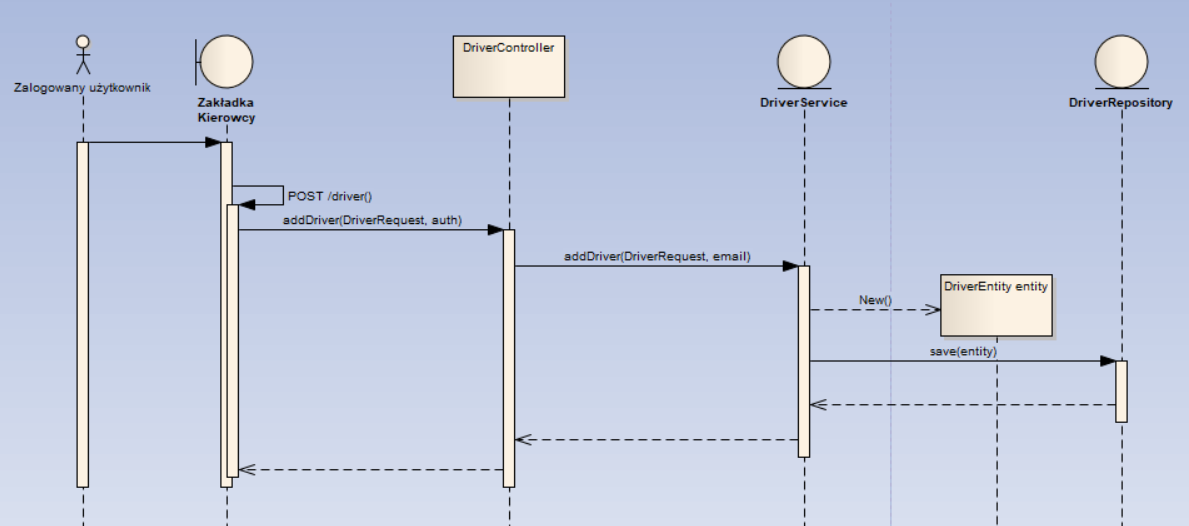
\includegraphics[width=1\textwidth]{./graf/sequence_diagram.png}
	\caption{Diagram sekwencji - dodanie kierowcy.}
	\label{sequence_diagram}
\end{figure}

\section{Opis struktur danych}
\paragraph{}
Dane w kodzie języka Java są reprezentowane przez encje. Są to klasy posiadające pola - zmienne odzwierciedlające kolumny w tabelach w bazie danych. Ich obiekty są odwzorowaniem bazodanowych rekordów. Przykład kodu można zobaczyć na rys. \ref{fig:kod:encja}. Każda zmienna posiada adnotację (poprzedzoną znakiem "@"), jest to składania Hibernate. Dzięki temu jest możliwe mapowanie między obiektem encji, a rekordem w tabeli. Encje posiadają również funckje nazywane getterami - do pozyskiwania danych z konkretnych pól oraz setterami - do wpisywania wartości do pól.

\begin{figure}
\centering
\begin{lstlisting}
@Entity
@Table(name = "user", schema = "adm")
public class UserEntity {
  @Id
  @Column
  private String email;

  @Column
  private String password;

  @OneToMany(mappedBy = "user", fetch = FetchType.LAZY)
  private Set<DriverEntity> driver;

  public String getEmail() {
    return email;
  }

  public void setEmail(String username) {
    this.email = username;
  }

  public String getPassword() {
    return password;
  }

  public void setPassword(String password) {
    this.password = password;
  }

  public Set<DriverEntity> getDriver() {
    return driver;
  }

  public void setDriver(Set<DriverEntity> driver) {
    this.driver = driver;
  }
}
\end{lstlisting}
\caption{Kod encji użytkownika - Java.}
\label{fig:kod:encja}
\end{figure}

\paragraph{}
Aby wysyłać i odbierać dane od tzw. frontendu, czyli części aplikacji dotyczącej interfejsu użytkownika, niezbędne są klasy reprezentujące żądania (ang. request) - odbierane są przez kontrolery oraz odpowiedzi (ang. response) - wysyłane dane do części z językiem TypeScript. Zazwyczaj mają pola analogiczne do encji. Posiadają również funkcje pobierające wartości z konkretynch zmiennych oraz zapisujące wartości do nich, tak jak jest to w przypadku encji. Odpowiedzi są również wyposażone w funkcje konwertujące obiekt encji na obiekt odpowiedzi. Przykład klasy żądania znajduje się na rys. \ref{fig:kod:request}, a metody do konwersji, będącej w klasie odpowiedzi, na rys. \ref{fig:kod:mapper}

\begin{figure}
\centering
\begin{lstlisting}
public class UserRequest {

    @NotNull
    private String email;
    
    @NotNull
    private String password;

    public String getEmail() {
        return email;
    }

    public void setEmail(String email) {
        this.email = email;
    }

    public String getPassword() {
        return password;
    }

    public void setPassword(String password) {
        this.password = password;
    }
}
\end{lstlisting}
\caption{Kod żądania użytkownika.}
\label{fig:kod:request}
\end{figure}

\begin{figure}
\centering
\begin{lstlisting}
public static TrackerResponse fromEntity(TrackerEntity entity){
        TrackerResponse dto = new TrackerResponse();
        dto.setSerialNumber(entity.getSerialNumber());
        dto.setName(entity.getName());
        dto.setType(entity.getType());
        return dto;
    }
\end{lstlisting}
\caption{Funkcja konwertująca encję na odpowiedź.}
\label{fig:kod:mapper}
\end{figure}

\paragraph{}
Analogiczne typy danych zostały stworzone w języku TypeScript w formie interfejsów, pozwalają one w prosty sposób wysyłać żądania i odbierać odpowiedzi. Posiadają one zmienne o identycznych nazwach co klasy w języku Java oraz typy, które pozwalają na automatyczne ich konwertowanie między językami podczas wysyłania i odbierania żądań HTTP. Wygląd interfejsów przedstawia rys. \ref{fig:kod:dto}.

\begin{figure}
\centering
\begin{lstlisting}
export interface UserRequest {
  email: string | null;
  password: string | null;
}
\end{lstlisting}
\caption{Kod żądania użytkownika - TypeScript.}
\label{fig:kod:dto}
\end{figure}

\section{Model danych}
\paragraph{}
Schemat bazy danych znajduje się na rys. \ref{fig:database}. Podstawową tabelą jest tabela użytkownika ("user") - przechowuje ona dane użytkowników systemu. Aplikacja umożliwia dodanie wielu kierowców, pojazdów i lokalizatorów, dlatego tabele: "drivers", "vehicles" oraz "trackers" są powiązane z użytkownikiem relacjami N:1. Dzięki temu jest możliwe wyświetlanie użytkownikowi odpowiednich pozycji w listach, gdyż każdy obiekt jest przypisany do konkretnego użytkownika. Tabela "location" przechowuje dane geograficzne zebrane od urządzeń GPS. Dzięki powiązaniu z tabelą lokalizatorów, można uzyskać łatwy dostęp do historii położenia danego urządzenia. Aby uzyskać dostęp do trasy przebytej przez samochód, niezbędne jest powiązanie między lokalizatorem, a pojazdem reprezentowane przez tabelę "vehicle\_tracker". Analogiczne powiązanie - pojazdu z kierowcą ("vehicle\_driver") - umożłiwia otrzymanie danych lokalizacyjnych dla konkretnego kierowcy.

\begin{figure}
	\centering
	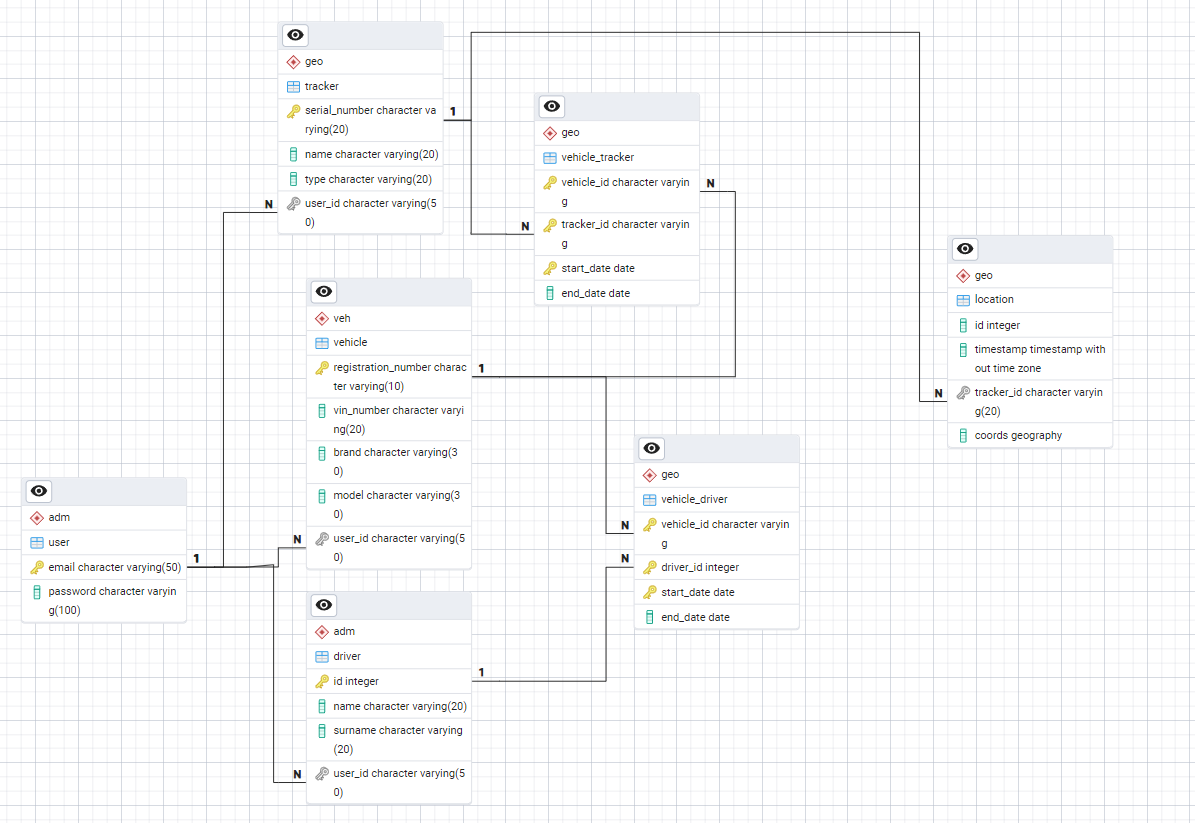
\includegraphics[width=1\textwidth]{./graf/database.png}
	\caption{Schemat bazy danych.}
	\label{fig:database}
\end{figure}

\section{Szczegóły implementacji wybranych fragmentów}

\subsection{Komponenty React}
\paragraph{}
Do stworzenia interfejsu użytkownika wykorzystano komponenty funkcyjne z biblioteki React. Każda zakładka aplikacji posiada oddzielny komponent - każdy w osobnym pliku. Zwracają one JSX, czyli kod zbliżony do HTML, w którym można zagnieżdżać inne elementy. Niemniej jednak, należy pamiętać o zasadzie, iż zwrócić można tylko jeden element nadrzędny - to w nim można umieścić kolejne. Rys.\ref{fig:kod:jsx} pokazuje zwracany JSX przez zakładkę strony głównej (tekst z elementów <p> zostął wycięty).

\begin{figure}
\centering
\begin{lstlisting}
return (
    <div className="main-container">
      <h1 className="welcome-title">Witaj w GeoApp</h1>
      <p className="text description1">
      </p>
      <p className="text description2">
      </p>
    </div>
 );
\end{lstlisting}
\caption{Zwracany JSX przez zakładkę strony głównej.}
\label{fig:kod:jsx}
\end{figure}


Ważnym elementem stworzonej aplikacji są formularze, to dzięki nim użytkownik dodaje obiekty czy powiązania. W tym celu została wykorzystana biblioteka React Hook Form, dostępna w React. Stworzono typy danych, którego przykład można zobaczyć na rys. \ref{fig:kod:formType}. Aby skorzystać z bibblioteki, wykorzystano Hook do destrukturyzacji niezbędnych stałych (rys. \ref{fig:kod:consts}). Aby skorzystać z obsługi formularza, zarejestrowano pola oraz dodano walidacje - przykład na rys. \ref{fig:kod:register}.

\begin{figure}
\centering
\begin{lstlisting}
type FormState = {
  name: string;
  surname: string;
};
\end{lstlisting}
\caption{Typ danych do formularza.}
\label{fig:kod:formType}
\end{figure}

\begin{figure}
\centering
\begin{lstlisting}
const [formState, setFormState] = useState<string>("addDriver");
  const {
    register,
    handleSubmit,
    formState: { errors },
    reset,
  } = useForm<FormState>();
\end{lstlisting}
\caption{Destrukturyzacja stałych z biblioteki React Hook Form.}
\label{fig:kod:consts}
\end{figure}

\begin{figure}
\centering
\begin{lstlisting}
<label className="form-label" htmlFor="name">Imie</label>
<input
  className="form-input"
  id="name"
  {...register("name", { required: "Imie jest wymagane" })}
/>
{errors.name && <p className="form-error form-validation-text">{errors.name.message}</p>}
\end{lstlisting}
\caption{Rejestracja i walidacja pól.}
\label{fig:kod:register}
\end{figure}

Mapa została zaimplementowana przy uzyciu biblioteki Leaflet. Inicjalizacja mapy następuje w useEffect(), czyli w funkcji React, która dzięki pustej tablicy zależności, znajdującej się na samym końcu, wykonuje się raz, gdy komponent mapy zostaje stworzony. Inicjalizację przedstawia rys. \ref{fig:kod:mapInit}. W celu wyświetlania tras na mapie, wykorzystano funkcję polyline(), która łączy linią kolejne punkty, przekazane jako argument w formie tablicy. Ta część kodu widnieje na rys. \ref{fig:kod:polyline}. Utworzona trasa zostaje dodana do mapy. 

\begin{figure}
\centering
\begin{lstlisting}
useEffect(() => {
    if (!mapRef.current && document.getElementById("map")) {
      mapRef.current = leaflet.map("map").setView([50.299, 18.787], 13);

      leaflet
        .tileLayer("https://tile.openstreetmap.org/{z}/{x}/{y}.png", {
          maxZoom: 19,
          attribution:
            '&copy; <a href="http://www.openstreetmap.org/copyright">OpenStreetMap</a>',
        })
        .addTo(mapRef.current);
    }
    loadTrackerData();
    loadVehicleData();
    loadDriverData();

    return () => {
      mapRef.current?.remove();
      mapRef.current = null;
    };
  }, []);
\end{lstlisting}
\caption{Inicjalizacja mapy.}
\label{fig:kod:mapInit}
\end{figure}

\begin{figure}
\centering
\begin{lstlisting}
useEffect(() => {
    if (!mapRef.current) return;
  
    mapRef.current.eachLayer((layer) => {
      if (layer instanceof leaflet.Polyline) {
        mapRef.current?.removeLayer(layer);
      }
    });
  
    const latLngs: [number, number][] = locations
      .filter(loc => loc.latitude !== null && loc.longitude !== null)
      .map(loc => [loc.latitude as number, loc.longitude as number]);
  
    if (latLngs.length > 1) {
      leaflet.polyline(latLngs, { color: "blue", weight: 4 }).addTo(mapRef.current!);
    }
  }, [locations]);
\end{lstlisting}
\caption{Dodanie trasy do mapy.}
\label{fig:kod:polyline}
\end{figure}


\subsection{Proces generowania i obsługi żądań}
\paragraph{}
Pierwszym etapem jest wywołanie w komponencie React funkcji wysyłającej żądanie HTTP. Przykładowym procesem będzie pobranie listy kierowców danego użytkownika. Na rys. \ref{fig:kod:startRequest} wywołana zostaje funkcja getDrivers(), której implementację przedstawia rys. \ref{fig:kod:getDrivers}. Jest to funkcja w języku TypeScript, która umożliwia wysłanie żądania z wykorzystaniem metody GET, na bazowy URL z punktem końcowym "/driver". Następnym krokiem jest odebranie żądania w kontolerze, czyli przez część funkcjonalną aplikacji. Implementacja metody kontrolera związana z pobraniem listy kierowców znajduje się na rys. \ref{fig:kod:controlerGetDrivers}. Za logikę jest odpowiedzialny serwis, stąd metoda widniejąca w kontrolerze jest niewielkich rozmiarów. Niemniej jednak, warto zwrócić uwagę na argument o nazwie "auth" - on pobiera dane obecnie zalogowanego użytkownika, które są niezbędne do znalezienia odpowiednich kierowców. Serwis wykorzystuje repozytorium do wyszukania odpowiednich danych z bazy danych - co można zaobserować na rys. \ref{fig:kod:serviceGetDrivers}, a następnie zwraca listę kierowców, która przez kontroler jest wysyłana jako odpowiedź. Ostatecznie te dane trafiają do komponentu React.


\begin{figure}
\centering
\begin{lstlisting}
const loadDriverData = async () => {
    const data = await getDrivers();
    setDrivers(data);
  };
\end{lstlisting}
\caption{Wywołanie funkcji "getDrivers()", wysyłającej żądanie HTTP.}
\label{fig:kod:startRequest}
\end{figure}

\begin{figure}
\centering
\begin{lstlisting}
export async function getDrivers(): Promise<DriverResponse[] | null> {
    try {
        const response = await request("GET", "/driver");
        return response.data;
    } catch (error) {
        console.error("Error getting drivers:", error);
        return null;
    }
}
\end{lstlisting}
\caption{Kod funkcji wysyłającej żądanie HTTP w celu pobrania listy kierowców.}
\label{fig:kod:getDrivers}
\end{figure}

\begin{figure}
\centering
\begin{lstlisting}
@GetMapping("")
public ResponseEntity<DriverResponse[]> getDrivers(Authentication auth) {
     UserResponse user = (UserResponse) auth.getPrincipal();
     return ResponseEntity.ok(driverService.getDrivers(user.getEmail()));
}
\end{lstlisting}
\caption{Metoda kontrolera, pobierająca listę kierowców.}
\label{fig:kod:controlerGetDrivers}
\end{figure}

\begin{figure}
\centering
\begin{lstlisting}
@Transactional
public DriverResponse[] getDrivers(String email) {
    return driverRepository.findAllByUserEmail(email).stream()
            .map(DriverResponse::fromEntity)
            .toArray(DriverResponse[]::new);
}
\end{lstlisting}
\caption{Metoda serwisu, pobierająca listę kierowców.}
\label{fig:kod:serviceGetDrivers}
\end{figure} % [Właściwy dla kierunku -- np. Specyfikacja wewnętrzna]

% TODO
\chapter{Weryfikacja i walidacja}
\label{ch:06}

\section{Sposób testowania}
\paragraph{}
Aby przetestować działanie serwera oraz prawidłowość w konfiguracji lokalizatora wykorzystano maszynę wirtualną z systemem Linux Ubuntu, która posiadała publiczny adres IP. Zakupiono lokalizator Mking MK07A oraz kartę SIM z pakietem internetu oraz wysyłką wiadomości SMS. Następnie urządzenie zostało skonfigurowany poprzez SMS-y tak, aby wysyłało dane na adres maszyny wirtualnej z użyciem portu 8080. Jednak serwer w języku Java był dostępny na lokalnym komputerze stacjonarnym z systemem Windows. Aby przekierować pakiety na serwer, skorzystano z programu MobaXTerm, który umożliwia tunelowanie portów TCP. Kolejnym korkiem było zatrzymywanie serwera w odpowiednich miejscach w programie IntelliJ Idea, dzięki czemu następnie eliminowano błędy wynikające z niewłaściwej interpretacji pakietów oraz poprawiano kod serwera.

\paragraph{}
W celu sprawdzenia aplikacji pod kątem błędów przechodzono przez jej zakładki, a w nich przez formularze. Testowano ich pola oraz czy zostają one przesłane, podczas gdy brakuje wymaganych pól.

\section{Wykryte i usunięte błędy}
\paragraph{}
Podczs testów aplikacji wykryto, że formularze pozwalają wpisać w pola dat zakończenia daty wcześniejsze niż te będące już w polach dat rozpoczęcia. Rozwiązano ten błąd poprzez wprowadzenie walidacji na pola z datami, aby data do była musiala być późniejszą datą niż data od.

 % Weryfikacja i walidacja

% TODO
\chapter{Podsumowanie i wnioski}

\section{Uzyskane wyniki w świetle postawionych celów i zdefiniowanych wymagań}
\paragraph{}
Aplikacja została napisana zgodnie z wymaganiami, które zostały przedstawione. Odpowiednio skonfigurowany lokalizator - co ułatwia instrukcja dostępna w programie - poprawnie współpracuje z serwerem, w wyniku czego można korzystać z aplikacji w sposób zgodny z początkowymi celami. Prosty interfejs pozwala użytkownikowi na sprawne i przyjemne obsługiwanie programu. Widok został dostosowany do różnej wielkości ekranów, co wskazuje na sukces podczas wprowadzania skalowalności. Wszystkie operacje, które miały być dostępne do wykonania przez użytkownika, i które miały na celu osiągnięcie użytecznej aplikacji, zostały wprowadzone.

\section{Kierunek ewentualnych prac}
\paragraph{}
Dalszym etapem rozwijania aplikacji byłoby przede wszystkim zwiększenie dostępnych typów lokalizatorów, wspieranych przez program. W tym celu należy rozbudować kod serwera, odbierającego dane geograficzne od urządzeń. Przykładem innego lokalizatora jest Coban TK108, który również umożliwia wysyłanie pakietów TCP na niestandardowy adres IP oraz port. Takie działania zwiększyłyby grupę potencjalnych użytkowników aplikacji, gdyż nie byliby oni ograniczeni do zakupu jednego modelu lokalizatora.
 % Podsumowanie i wnioski

\backmatter

%\bibliographystyle{plplain}  % bibtex
%\bibliography{biblio/biblio} % bibtex
\printbibliography           % biblatex
\addcontentsline{toc}{chapter}{Bibliografia}

\begin{appendices}

% TODO
\chapter{Spis skrótów i symboli}

\begin{itemize}
\item[DNA] kwas deoksyrybonukleinowy (ang. \english{deoxyribonucleic acid})
\item[MVC] model -- widok -- kontroler (ang. \english{model--view--controller}) 
\item[$N$] liczebność zbioru danych
\item[$\mu$] stopnień przyleżności do zbioru
\item[$\mathbb{E}$] zbiór krawędzi grafu
\item[$\mathcal{L}$] transformata Laplace'a 
\end{itemize}
 % Spis skrótów i symboli

% TODO
\chapter{Źródła}

Jeżeli w pracy konieczne jest umieszczenie długich fragmentów kodu źródłowego, należy je przenieść w to miejsce.

\begin{lstlisting}
if (_nClusters < 1)
	throw std::string ("unknown number of clusters");
if (_nIterations < 1 and _epsilon < 0)
	throw std::string ("You should set a maximal number of iteration or minimal difference -- epsilon.");
if (_nIterations > 0 and _epsilon > 0)
	throw std::string ("Both number of iterations and minimal epsilon set -- you should set either number of iterations or minimal epsilon.");
\end{lstlisting}


% % % % % % % % % % % % % % % % % % % % % % % % % % % % % % % % % % % 
% Pakiet minted wymaga odkomentowania w pliku config/settings.tex   %
% importu pakietu minted: \usepackage{minted}                       %
% i specjalnego kompilowania:                                       %
% pdflatex -shell-escape praca                                      %
% % % % % % % % % % % % % % % % % % % % % % % % % % % % % % % % % % % 

%\begin{minted}[linenos,breaklines,frame=lines]{c++}
%if (_nClusters < 1)
%   throw std::string ("unknown number of clusters");
%if (_nIterations < 1 and _epsilon < 0)
%   throw std::string ("You should set a maximal number of iteration or minimal difference -- epsilon.");
%if (_nIterations > 0 and _epsilon > 0)
%   throw std::string ("Both number of iterations and minimal epsilon set -- you should set either number of iterations or minimal epsilon.");
%\end{minted}
 % Źródła

% TODO
\chapter{Lista dodatkowych plików, uzupełniających tekst pracy} 


W systemie do pracy dołączono dodatkowe pliki zawierające:
\begin{itemize}
\item źródła programu,
\end{itemize}
 % Lista dodatkowych plików, uzupełniających tekst pracy

\listoffigures
\addcontentsline{toc}{chapter}{Spis rysunków}
\listoftables
\addcontentsline{toc}{chapter}{Spis tabel}

\end{appendices}

\end{document}


%% Finis coronat opus.

